\input{../utils/preamble}
\createdgmtitle{supp}
%--------------------------------------------------------------------------------
\begin{document}
%--------------------------------------------------------------------------------
\begin{frame}
%\thispagestyle{empty}
\titlepage
\end{frame}
%=======
\begin{frame}{GatedPixelCNN}
\end{frame}
%=======
\begin{frame}{GatedPixelCNN (2016)}
\begin{figure}
	\centering
	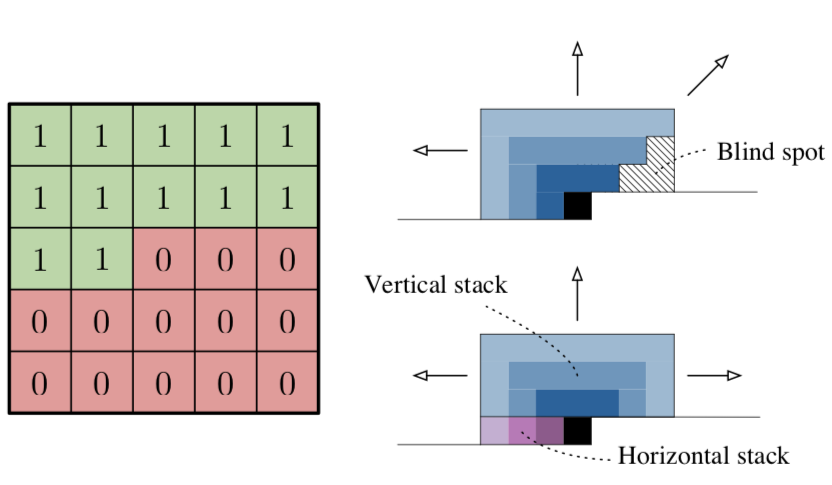
\includegraphics[width=0.5\linewidth]{figs/gatedpixelcnn.png}
	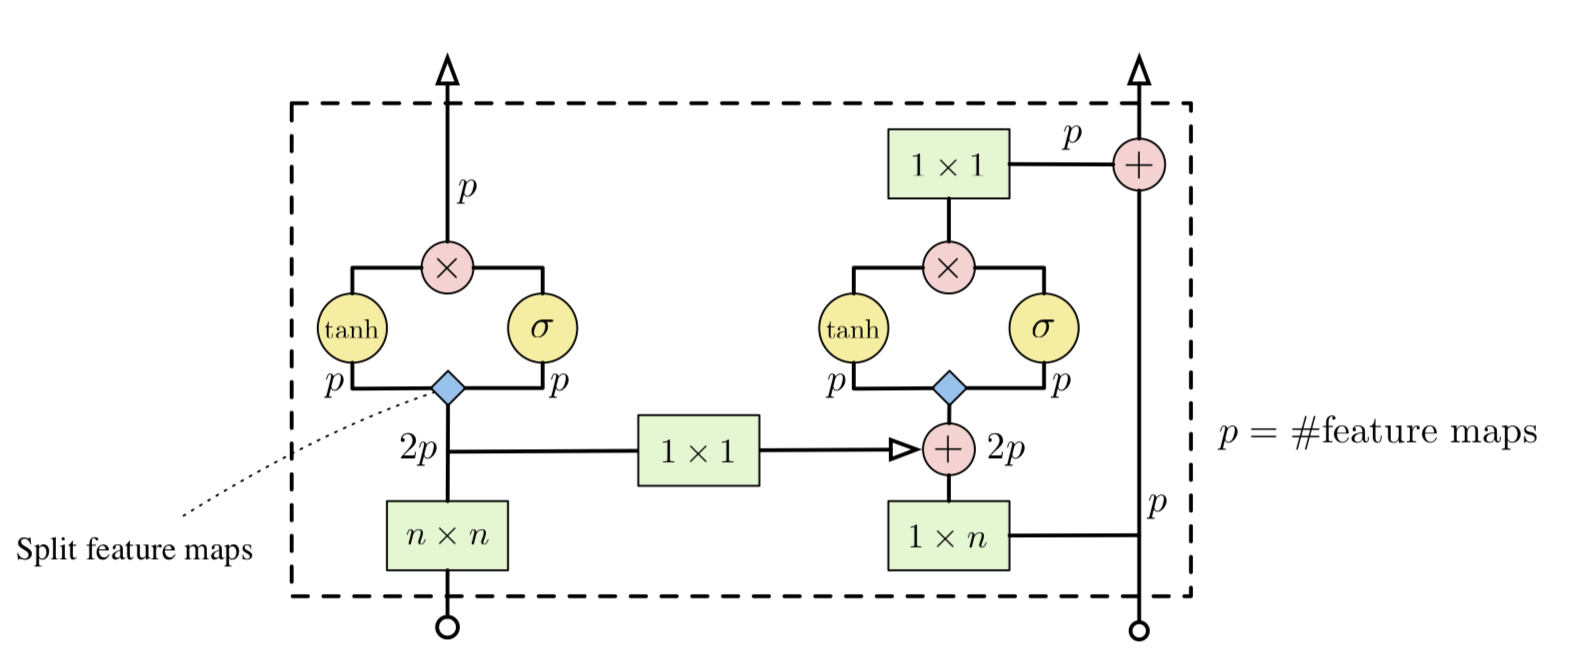
\includegraphics[width=0.5\linewidth]{figs/gated_block.png}
\end{figure}
\vfill
\hrule\medskip
{\scriptsize Van den Oord A. et al. Conditional image generation with pixelcnn decoders \href{https://arxiv.org/pdf/1606.05328.pdf}{https://arxiv.org/pdf/1606.05328.pdf}}
\end{frame}
%=======
\begin{frame}{GatedPixelCNN (2016)}
\begin{minipage}[t]{0.5\columnwidth}
	\begin{figure}[h]
		\centering
		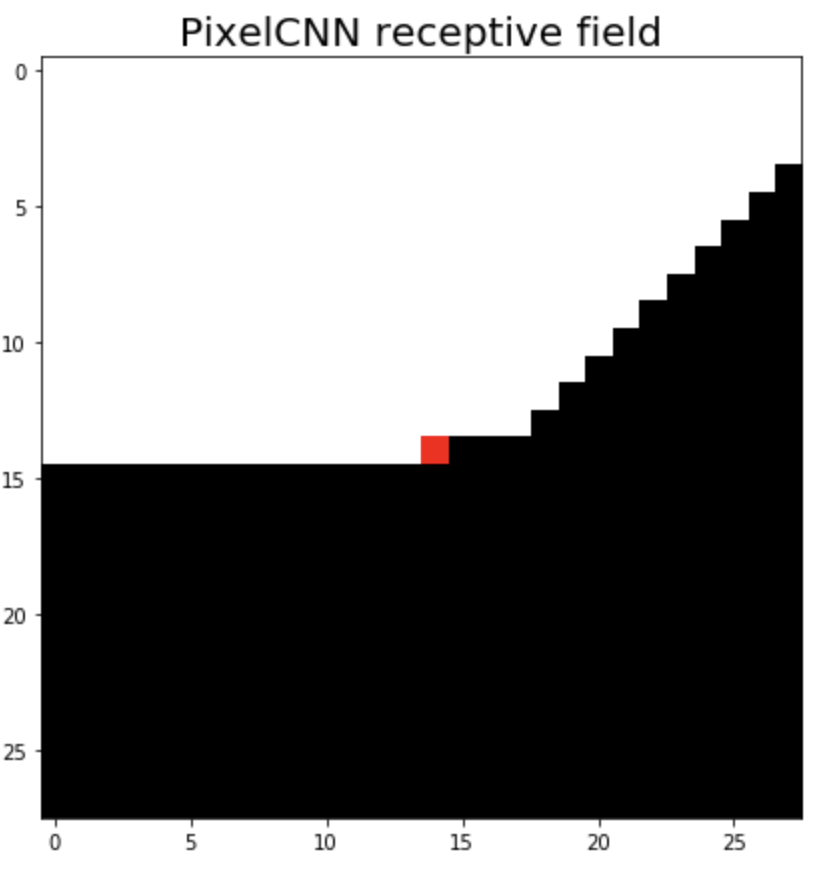
\includegraphics[width=0.9\linewidth]{figs/pixelcnn_receptive_field.png}
	\end{figure}
\end{minipage}%
\begin{minipage}[t]{0.5\columnwidth}
	\begin{figure}[h]
		\centering
		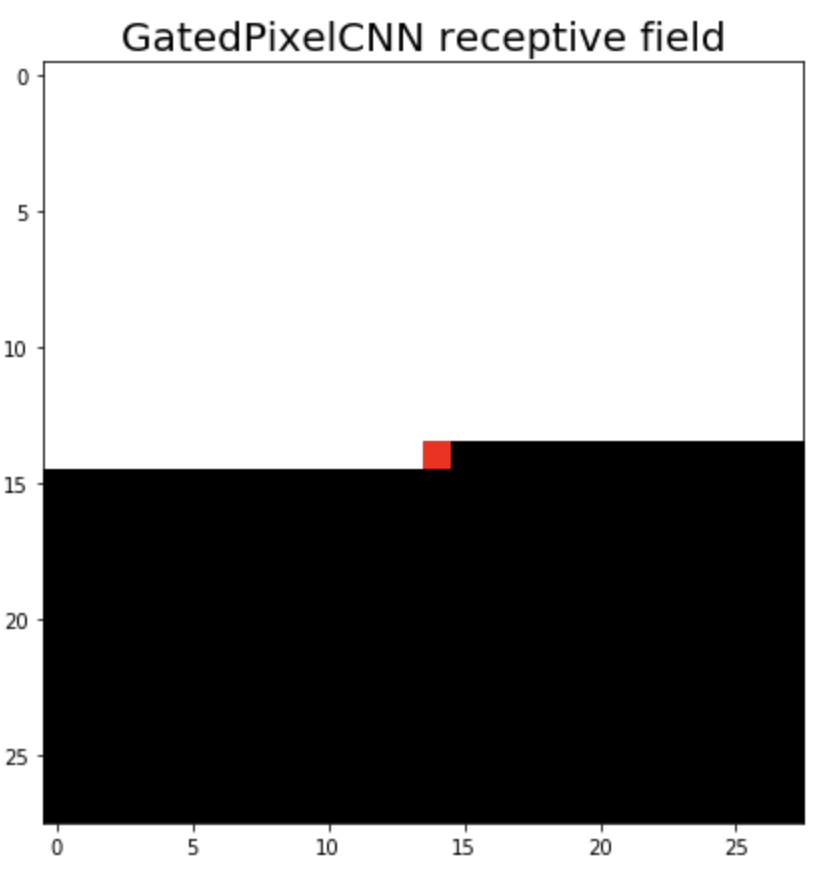
\includegraphics[width=0.9\linewidth]{figs/gatedpixelcnn_receptive_field.png}
	\end{figure}
\end{minipage}
\vfill
\hrule\medskip
{\scriptsize Van den Oord A. et al. Conditional image generation with pixelcnn decoders \href{https://arxiv.org/pdf/1606.05328.pdf}{https://arxiv.org/pdf/1606.05328.pdf}}
\end{frame}
%=======
\begin{frame}{Extensions}
\begin{itemize}
	\item \textbf{PixelCNN++}: \textit{Improving the PixelCNN with Discretized Logistic Mixture Likelihood and Other Modifications} \\
	\href{https://arxiv.org/pdf/1701.05517.pdf}{https://arxiv.org/pdf/1701.05517.pdf} \\
	(mixture of logistics instead of softmax);
	\item \textbf{PixelSNAIL}: \textit{An Improved Autoregressive Generative Model} \\
	\href{https://arxiv.org/pdf/1712.09763.pdf}{https://arxiv.org/pdf/1712.09763.pdf} \\
	(self-attention to learn optimal autoregression ordering).
\end{itemize}
\end{frame}
%=======
\begin{frame}{ELBO gradient, Log derivative trick}
\end{frame}
%=======
\begin{frame}{ELBO gradient (E-step, $\nabla_{\bphi} \mathcal{L}(\bphi, \btheta)$)}
\vspace{-0.3cm}
\[
	\mathcal{L} (\bphi, \btheta)  = \mathbb{E}_{q} \log p(\bX | \bZ, \btheta) - KL (q(\bZ| \bX, \phi) || p(\bZ)) \rightarrow \max_{\bphi, \btheta}.
\]
	Difference from M-step: density function $q(\bz| \bx, \bphi)$ depends on the parameters $\bphi$, it is impossible to use Monte-Carlo estimation:
	\[
		\nabla_{\bphi} \mathcal{L} (\bphi, \btheta) = \int \nabla_{\bphi} q(\bZ| \bX, \bphi) \log p(\bX |\bZ, \btheta) d\bZ - \nabla_{\bphi} KL
	\]
	
	\begin{block}{Log-derivative trick}
	    \[
	    \nabla_\xi q(\eta| \xi) = q(\eta | \xi) \left( \frac{\nabla_\xi q(\eta | \xi)}{q(\eta| \xi)} \right) = q(\eta | \xi) \nabla_\xi \log q(\eta| \xi).
	    \]
	\end{block}
	\[
		\nabla_{\bphi} q(\bZ| \bX, \bphi) = q(\bZ| \bX, \bphi) \nabla_{\bphi} \log q(\bZ| \bX, \bphi).
	\]
\end{frame}
%=======
\begin{frame}{ELBO gradient (E-step, $\nabla_{\bphi} \mathcal{L}(\bphi, \btheta)$)}

	\begin{multline*}
		\nabla_{\bphi} \mathcal{L} (\bphi, \btheta) = \int \nabla_{\bphi} q(\bZ| \bX, \bphi) \log p(\bX |\bZ, \btheta) d\bZ  - \nabla_{\bphi} KL = \\ 
		=  \int q(\bZ| \bX, \bphi) \bigl[  \nabla_{\bphi} \log q(\bZ| \bX, \bphi) \log p(\bX |\bZ, \btheta) \bigr] d\bZ - \nabla_{\bphi} KL
	\end{multline*}
	After applying log-reparametrization trick, we are able to use Monte-Carlo estimation:
	\[
		\nabla_{\bphi} \mathcal{L} (\bphi, \btheta) \approx n \nabla_{\bphi} \log q(\bz_i^*| \bx_i, \bphi) \log p(\bx_i |\bz_i^*, \btheta) - \nabla_{\bphi} KL,
	\]
	\[
		\bz_i^* \sim q(\bz_i| \bx_i, \bphi).
	\]
	\vspace{-0.2cm}
	\begin{block}{Problem} 
	Unstable solution with huge variance.
	\end{block}
	\begin{block}{Solution}
	    Reparametrization trick
	\end{block}
\end{frame}
%=======
\begin{frame}{IWAE, active units, posterior collapse}
\end{frame}
%=======
\begin{frame}{IWAE, 2015}
How to determine whether all VAE latent variables are informative?
\[
A_{i} = \text{cov}_\bx \left( \mathbb{E}_{q(z_i | \bx)} [z_i] \right) > 0.01 \quad \Leftrightarrow \quad z_i \text{ is active}
\]
\begin{figure}
	\centering
	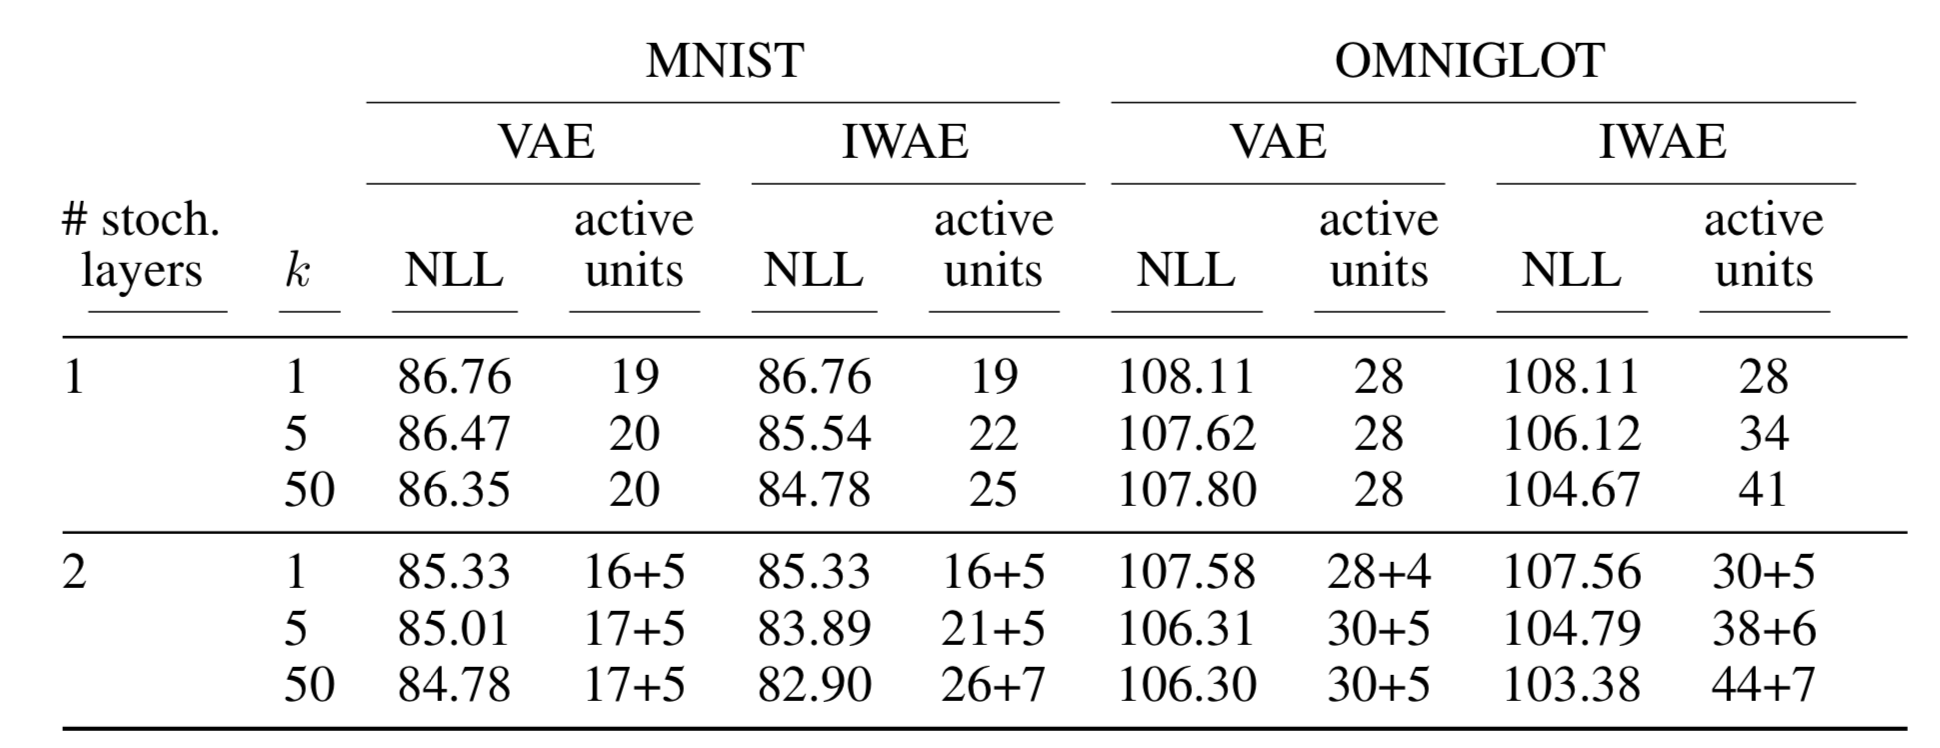
\includegraphics[width=\linewidth]{figs/IWAE_3.png}
\end{figure}
\vfill
\hrule\medskip
{\scriptsize \href{https://arxiv.org/pdf/1509.00519.pdf}{https://arxiv.org/pdf/1509.00519.pdf}}
\end{frame}
%=======
\begin{frame}{PixelVAE, Hierarchical VAE}
\end{frame}
%=======
\begin{frame}{PixelVAE, 2016}
	\begin{block}{Hierarchical VAE}
		\begin{figure}
			\centering
			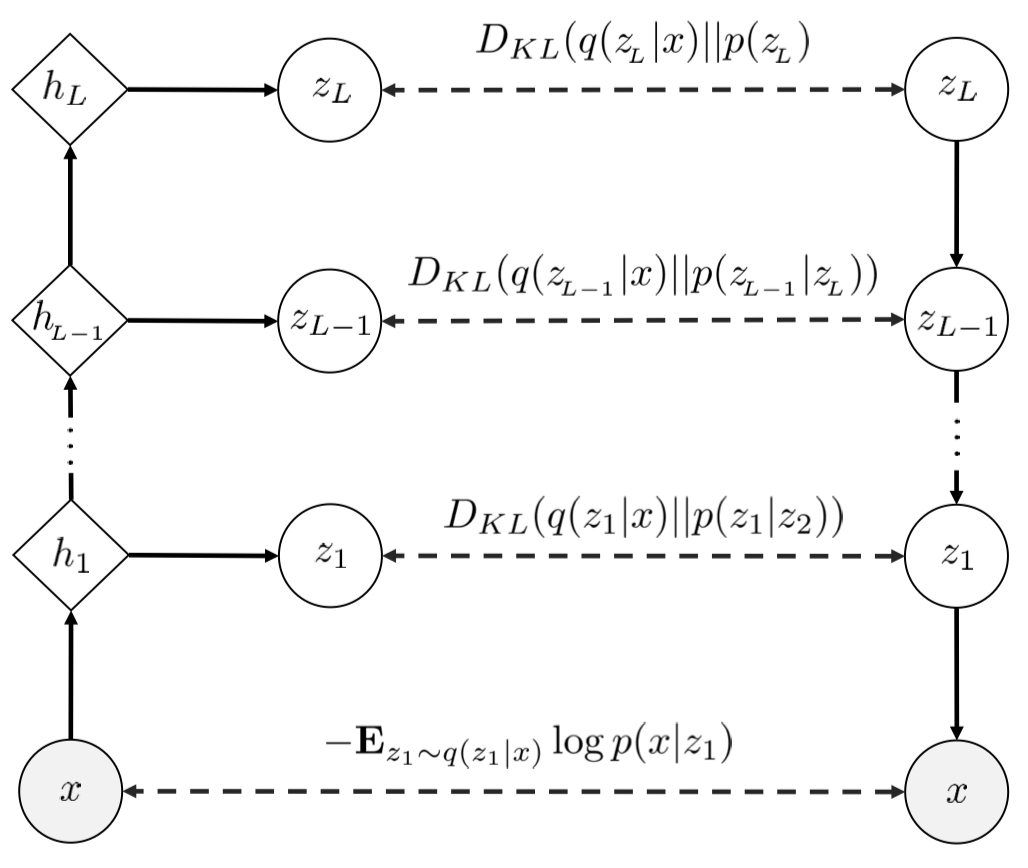
\includegraphics[width=0.7\linewidth]{figs/PixelVAE_1.png}
		\end{figure}
	\end{block}
	\vfill
	\hrule\medskip
	{\scriptsize \href{https://arxiv.org/pdf/1611.05013.pdf}{https://arxiv.org/pdf/1611.05013.pdf}}
\end{frame}
%=======
\begin{frame}{PixelVAE, 2016}
	\begin{block}{Hierarchical decomposition}
		\vspace{-1cm}
		\begin{align*}
			p(\bz_1, \dots, \bz_L) &= p(\bz_L) p(\bz_{L-1} | \bz_L) \dots p(\bz_1, \bz_2); \\
			q(\bz_1, \dots, \bz_L | \bx) &= q(\bz_1 | \bx) \dots q(\bz_L | \bx).
		\end{align*}
	\end{block}
	\vspace{-0.5cm}
	\begin{block}{ELBO}
		\vspace{-0.5cm}
		{\footnotesize
			\begin{align*}
				\mathcal{L}(q, \btheta) &= \mathbb{E}_{q(\bz_1 | \bx)} \log p(\bx | \bz_1, \btheta) - KL(q(\bz_1, \dots, \bz_L | \bx) || p(\bz_1, \dots, \bz_L)) \\
				&= \mathbb{E}_{q(\bz_1 | \bx)} \log p(\bx | \bz_1, \btheta) - \int \prod_{j=1}^L q(\bz_j | \bx) \sum_{i=1}^L \log \frac{q(\bz_i | \bx)}{p(\bz_i | \bz_{i + 1})} d \bz_1 \dots d \bz_L \\
				&= \mathbb{E}_{q(\bz_1 | \bx)} \log p(\bx | \bz_1, \btheta) - \sum_{i=1}^L \int \prod_{j=1}^L q(\bz_j | \bx) \log \frac{q(\bz_i | \bx)}{p(\bz_i | \bz_{i + 1})} d \bz_1 \dots d \bz_L \\
				&= \mathbb{E}_{q(\bz_1 | \bx)} \log p(\bx | \bz_1, \btheta) - \sum_{i=1}^L \int q(\bz_{i+1} | \bx) q(\bz_i | \bx) \log \frac{q(\bz_i | \bx)}{p(\bz_i | \bz_{i + 1})} d \bz_i d \bz_{i+1} \\
				&= \mathbb{E}_{q(\bz_1 | \bx)} \log p(\bx | \bz_1, \btheta) - \sum_{i=1}^L \mathbb{E}_{q(\bz_{i+1} | \bx)} \left[ KL (q(\bz_i | \bx) || p(\bz_i | \bz_{i + 1}))\right]
			\end{align*}
		}
	\end{block}
	\vfill
	\hrule\medskip
	{\scriptsize \href{https://arxiv.org/pdf/1611.05013.pdf}{https://arxiv.org/pdf/1611.05013.pdf}}
\end{frame}
%=======
\begin{frame}{RevNet, i-RevNet}
\end{frame}
%=======
\begin{frame}{RevNets, 2017}
	\begin{minipage}[t]{0.6\columnwidth}
		\begin{itemize}
			\item Modern neural networks are trained via backpropagation.
			\item Residual networks are state of the art in image classification.
			\item Backpropagation requires storing the network activations.
		\end{itemize}
	\end{minipage}%
	\begin{minipage}[t]{0.4\columnwidth}
		\begin{figure}
			\centering
			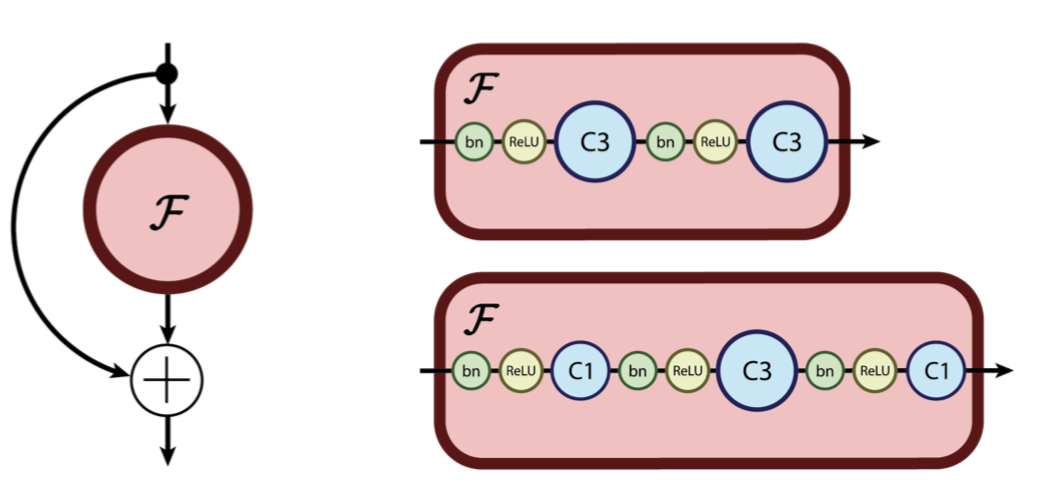
\includegraphics[width=\linewidth]{figs/resnet_block.png}
		\end{figure}
	\end{minipage}
	\vspace{0.1cm}
	\begin{block}{Problem}
		Storing the activations imposes an increasing memory burden. GPUs have limited memory capacity, leading to constraints often exceeded by state-of-the-art architectures (with thousand layers).
	\end{block}
	\myfootnotewithlink{https://arxiv.org/abs/1707.04585}{Gomez A. N. et al. The Reversible Residual Network: Backpropagation Without Storing Activations, 2017}
\end{frame}
%=======
\begin{frame}{RevNets, 2017}
	\begin{block}{NICE}
		\vspace{-0.2cm}
		\begin{equation*}
			\begin{cases} \bz_1 = \bx_1; \\ \bz_2 = \bx_2 + \mathcal{F}(\bx_1, \btheta);\end{cases}  \quad \Leftrightarrow \quad 
			\begin{cases} \bx_1 = \bz_1; \\ \bx_2 = \bz_2 - \mathcal{F}(\bz_1, \btheta).\end{cases} 
		\end{equation*}
		\vspace{-0.2cm}
	\end{block}
	\begin{block}{RevNet}
		\begin{equation*}
			\begin{cases} \by_1 = \bx_1 + \mathcal{F}(\bx_2, \btheta); \\ \by_2 = \bx_2 + \mathcal{G}(\by_1, \btheta);\end{cases} \quad \Leftrightarrow \quad 
			\begin{cases} \bx_2 = \by_2 - \mathcal{F}(\by_1, \btheta); \\ \bx_1 = \by_1 - \mathcal{G}(\bx_2, \btheta).\end{cases} 
		\end{equation*}
	\end{block}
	\begin{figure}
		\centering
		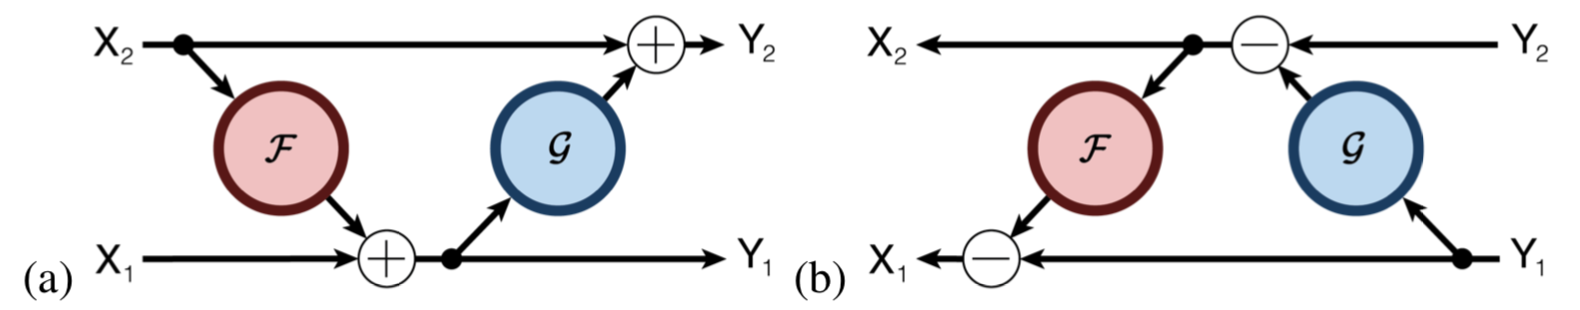
\includegraphics[width=\linewidth]{figs/revnet.png}
	\end{figure}
	\myfootnotewithlink{https://arxiv.org/abs/1707.04585}{Gomez A. N. et al. The Reversible Residual Network: Backpropagation Without Storing Activations, 2017}
\end{frame}
%=======
\begin{frame}{RevNets, 2017}
	\begin{figure}
		\centering
		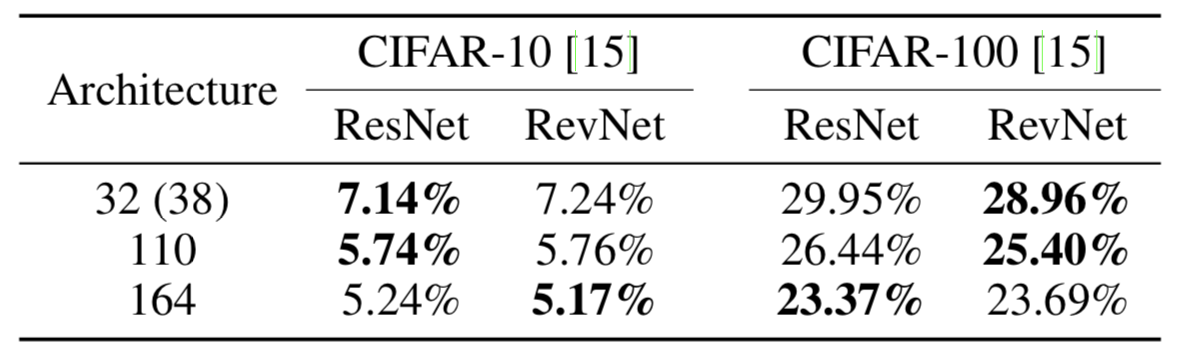
\includegraphics[width=0.8\linewidth]{figs/revnet_results.png}
	\end{figure}
	\begin{itemize}
		\item If the network contains non-reversible blocks (poolings, strides), activations for these blocks should be stored.
		\item To avoid storing activations in the modern frameworks, the backward pass should be manually redefined.
	\end{itemize}
	\myfootnotewithlink{https://arxiv.org/abs/1707.04585}{Gomez A. N. et al. The Reversible Residual Network: Backpropagation Without Storing Activations, 2017}
\end{frame}
%=======
\begin{frame}{i-RevNet, 2018}
	\begin{block}{Hypothesis}
		The success of deep convolutional networks is based on progressively discarding uninformative variability about the input with respect to the problem at hand. 
	\end{block}
	\begin{itemize}
		\item It is difficult to recover images from their hidden representations. 
		\item Information bottleneck principle: an optimal representation must reduce the MI between an input and its representation to reduce uninformative variability + maximize the MI between the output and its representation to preserve each class from collapsing onto other classes.
	\end{itemize}
	\myfootnotewithlink{https://arxiv.org/abs/1802.07088}{Jacobsen J. H., Smeulders A., Oyallon E. i-RevNet: Deep Invertible Networks, 2018}
\end{frame}
%=======
\begin{frame}{i-RevNet, 2018}
	\begin{block}{Hypothesis}
		The success of deep convolutional networks is based on progressively discarding uninformative variability about the input with respect to the problem at hand. 
	\end{block}
	
	\begin{block}{Idea}
		Build a cascade of homeomorphic layers (i-RevNet), a network that can be fully inverted up to the final projection onto the classes, i.e. no information is discarded.
	\end{block}
	\myfootnotewithlink{https://arxiv.org/abs/1802.07088}{Jacobsen J. H., Smeulders A., Oyallon E. i-RevNet: Deep Invertible Networks, 2018}
\end{frame}
%=======
\begin{frame}{i-RevNet, 2018}
	
	\begin{figure}
		\centering
		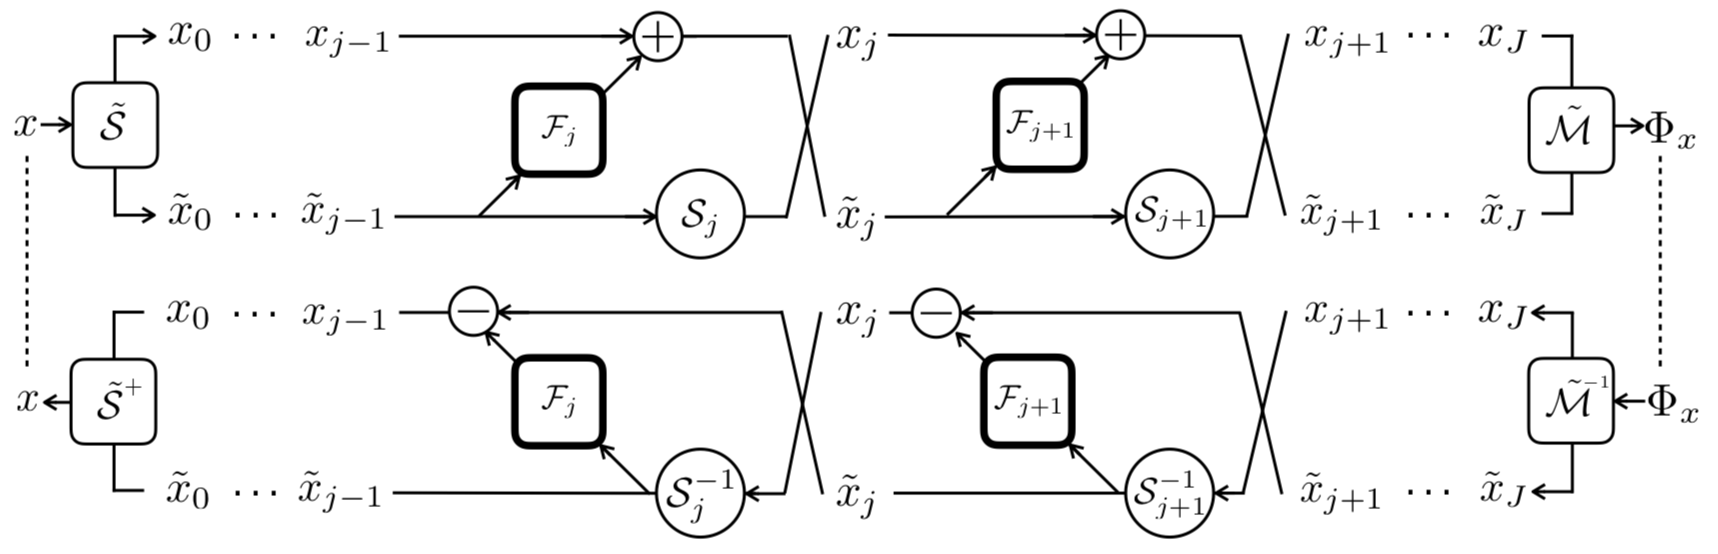
\includegraphics[width=\linewidth]{figs/i-revnet.png}
	\end{figure}
	
	\begin{figure}
		\centering
		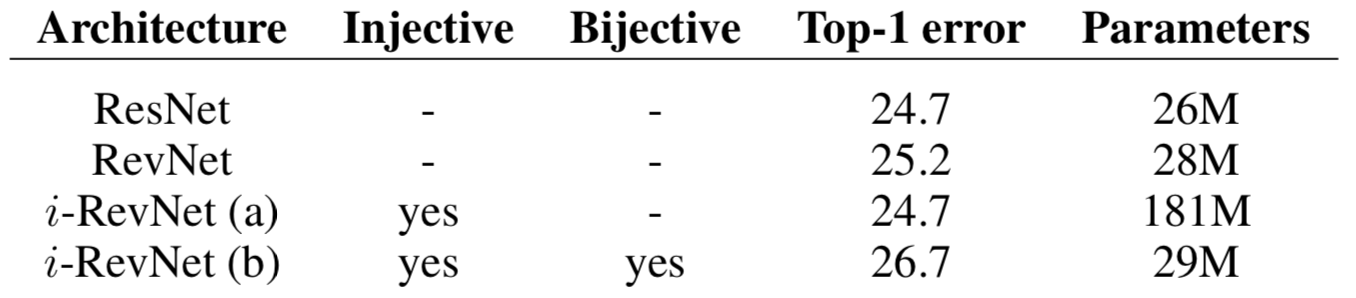
\includegraphics[width=0.9\linewidth]{figs/i-revnet_block.png}
	\end{figure}

	\myfootnotewithlink{https://arxiv.org/abs/1802.07088}{Jacobsen J. H., Smeulders A., Oyallon E. i-RevNet: Deep Invertible Networks, 2018}
\end{frame}
%=======
\begin{frame}{Posterior collapse, toy example}
\end{frame}
%=======
\begin{frame}{Posterior collapse: toy example}
	Let define latent variable model in the following way:
	\[
	p(\bx | \btheta) = \int p(\bx, \bz | \btheta) d \bz = \int p(\bx | \bz, \btheta) p(\bz) d \bz 
	\]
	\begin{itemize}
		\item prior distribution $p(\bz) = \mathcal{N}(\bz| 0, \mathbf{I})$;
		\item probabilistic model $p(\bx | \bz, \btheta) = \mathcal{N}(\bx | \bmu_{\btheta}(\bz), \bsigma_{\btheta}(\bz))$ (diagonal covariance);
		\item variational posterior $q(\bz | \bx, \bphi) =  \mathcal{N}(\bx | \bmu_{\bphi}(\bx), \bsigma_{\phi}(\bx))$  (diagonal covariance).
	\end{itemize}
	
	Let data distribution is $\pi(\bx) = \mathcal{N}(\bx | \bmu, \bSigma)$. Possible cases:
	\begin{itemize}
		\item covariance matrix $\bSigma$ is diagonal (univariate case);
		\item covariance matrix $\bSigma$ is \textbf{not} diagonal (multivariate case).
	\end{itemize}
	What is the difference?
\end{frame}
%=======
\begin{frame}{Posterior collapse: toy example}
	\begin{block}{Multivariate ($\bSigma$ is non-diagonal)}
		\vspace{-0.5cm}
		\begin{minipage}[t]{0.33\columnwidth}
			\begin{figure}[h]
				\centering
				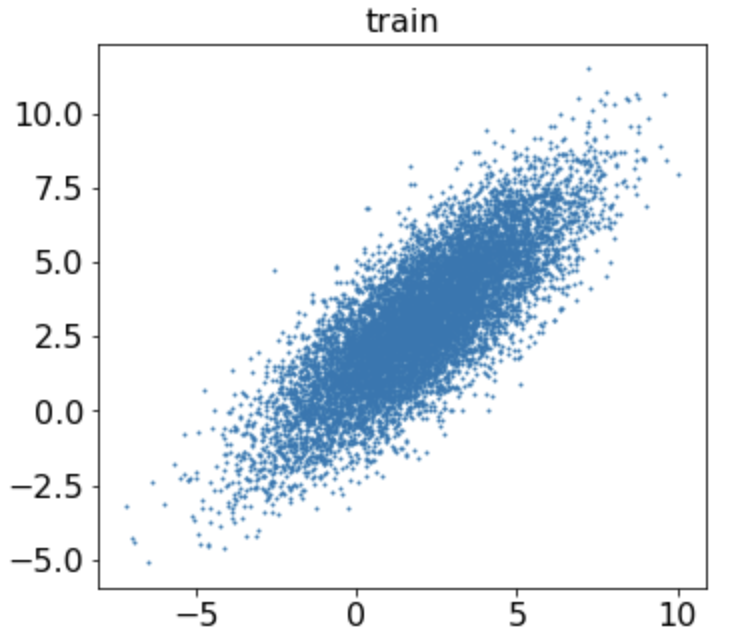
\includegraphics[width=.8\linewidth]{figs/posterior_collapse_toy_1.png}
			\end{figure}
		\end{minipage}%
		\begin{minipage}[t]{0.33\columnwidth}
			\begin{figure}[h]
				\centering
				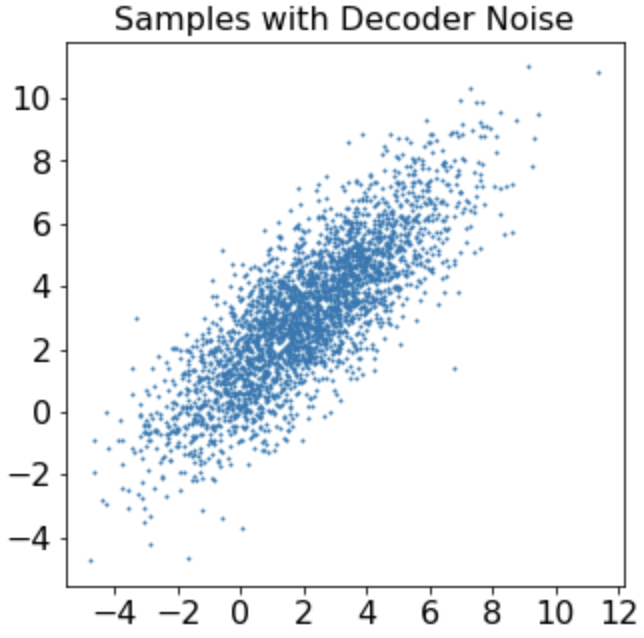
\includegraphics[width=0.75\linewidth]{figs/posterior_collapse_toy_3.png}
			\end{figure}
		\end{minipage}%
		\begin{minipage}[t]{0.33\columnwidth}
			\begin{figure}[h]
				\centering
				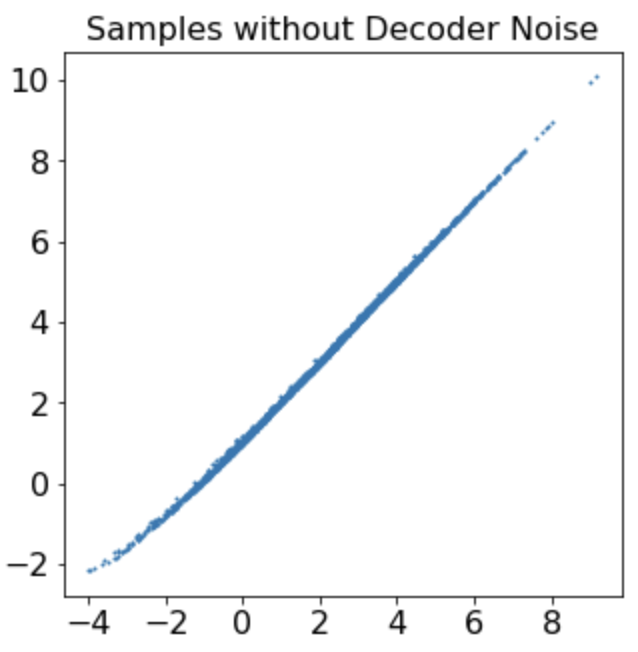
\includegraphics[width=.75\linewidth]{figs/posterior_collapse_toy_5.png}
			\end{figure}
		\end{minipage}
		The encoder uses latent variables to model data.
	\end{block}
	
	\begin{block}{Univariate ($\bSigma$ is diagonal)}
		\vspace{-0.5cm}
		\begin{minipage}[t]{0.33\columnwidth}
			\begin{figure}[h]
				\centering
				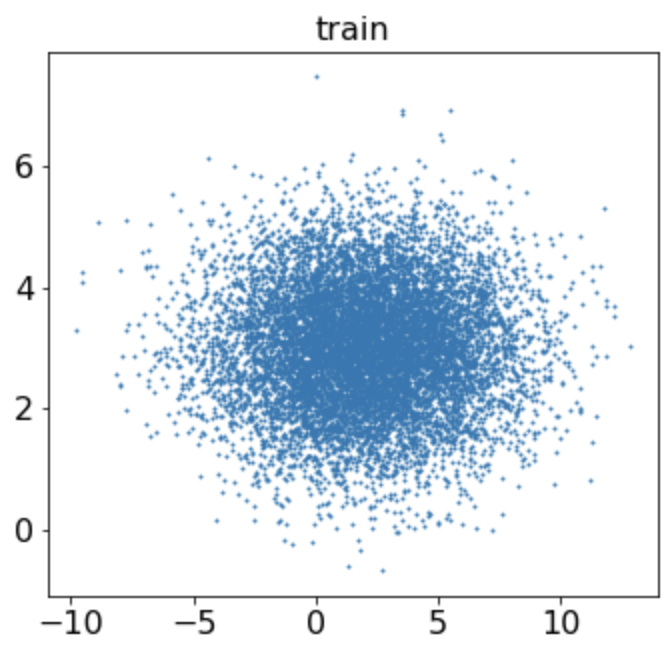
\includegraphics[width=.8\linewidth]{figs/posterior_collapse_toy_2.png}
			\end{figure}
		\end{minipage}%
		\begin{minipage}[t]{0.33\columnwidth}
			\begin{figure}[h]
				\centering
				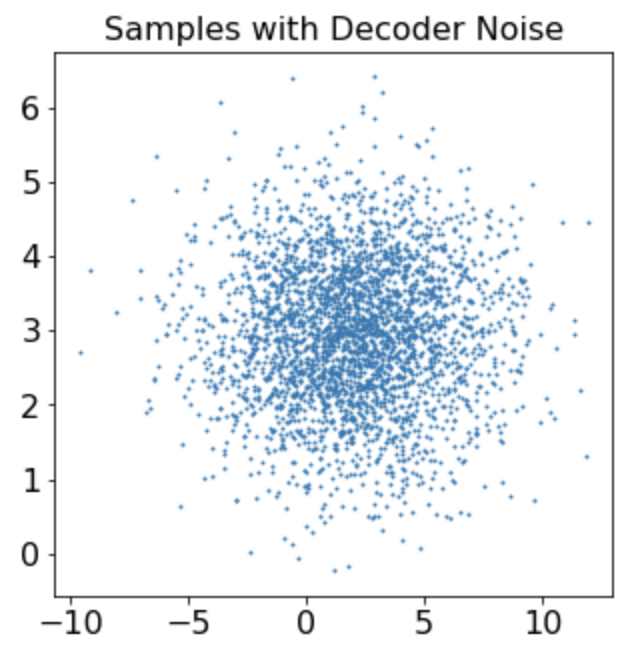
\includegraphics[width=.75\linewidth]{figs/posterior_collapse_toy_4.png}
			\end{figure}
		\end{minipage}%
		\begin{minipage}[t]{0.33\columnwidth}
			\begin{figure}[h]
				\centering
				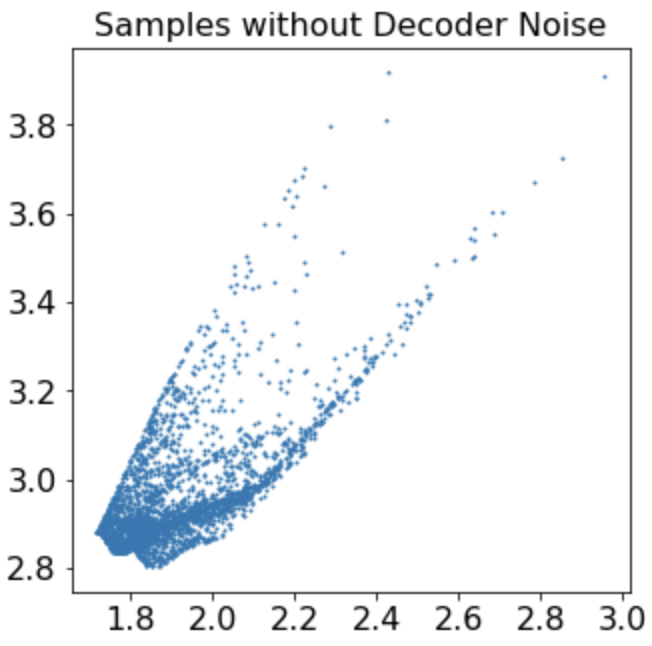
\includegraphics[width=.75\linewidth]{figs/posterior_collapse_toy_6.png}
			\end{figure}
		\end{minipage}
		Latent variables are not used, since the decoder could model the data without the encoder.
	\end{block}
\end{frame}
%=======
\begin{frame}{Posterior collapse, VLAE}
\end{frame}
%=======
\begin{frame}{Variational Lossy AutoEncoder}
	\begin{block}{Lossy code via explicit information placement}
		\[
		p(\bx | \bz, \btheta) = \prod_{i=1}^m p(x_i | \bz, \bx_{\text{WindowAround}(i)}, \btheta).
		\]
		\begin{itemize}
			\item WindowAround($i$) restricts the receptive field (it forbids to represent arbitrarily complex distribution over $\bx$ without dependence on $\bz$). 
			\item Local statistics of 2D images (texture) will be modeled by a small local window.
			\item Global structural information (shapes) is long-range dependency that can only be communicated through latent code $\bz$. 
		\end{itemize}
	\end{block}
	\myfootnotewithlink{https://arxiv.org/abs/1611.02731}{Chen X. et al. Variational Lossy Autoencoder, 2016}
\end{frame}
%=======
\begin{frame}{Variational Lossy AutoEncoder}
	\begin{itemize}
		\item Can VLAE learn lossy codes that encode global statistics?
		\item Does using AF priors improves upon using IAF posteriors as predicted by theory?
		\item Does using autoregressive decoding distributions improve density estimation performance?
	\end{itemize}
	\begin{minipage}[t]{0.5\columnwidth}
		\vspace{1cm}
		MNIST
		\begin{figure}[h]
			\centering
			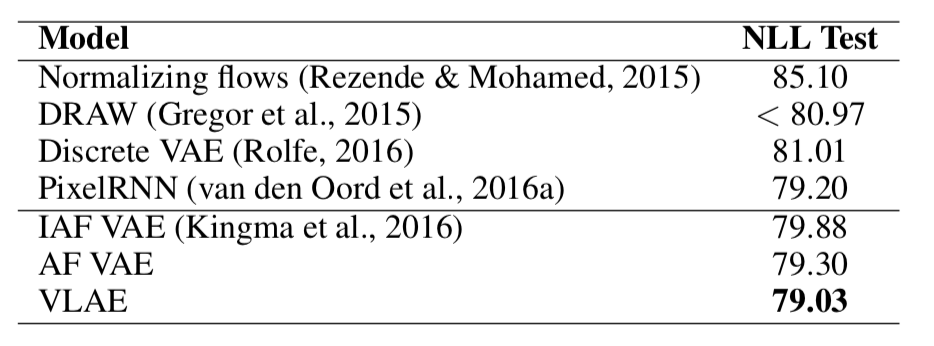
\includegraphics[width=1.\linewidth]{figs/VLAE_1.png}
		\end{figure}
	\end{minipage}%
	\begin{minipage}[t]{0.5\columnwidth}
		CIFAR10
		\begin{figure}[h]
			\centering
			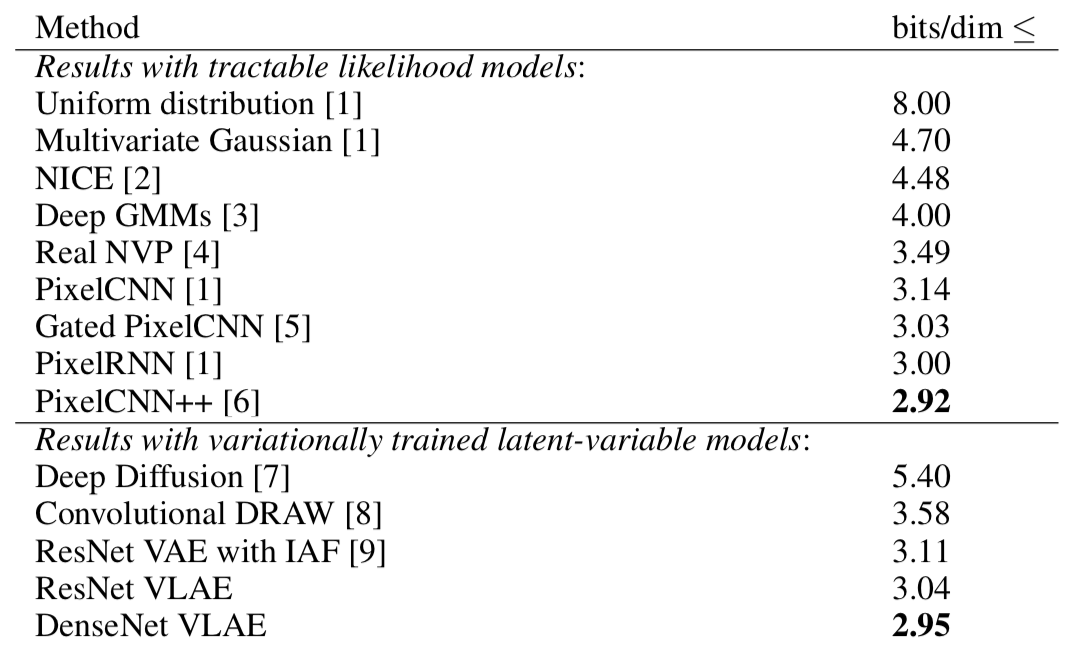
\includegraphics[width=1.\linewidth]{figs/VLAE_2.png}
		\end{figure}
	\end{minipage}
	
	\myfootnotewithlink{https://arxiv.org/abs/1611.02731}{Chen X. et al. Variational Lossy Autoencoder, 2016}
\end{frame}
%=======
\begin{frame}{Disentanglement, InfoGAN}
\end{frame}
%=======
\begin{frame}{InfoGAN}
	\begin{block}{GAN objective}
		\vspace{-0.6cm}
		\[
		\min_{G} \max_D V(G, D)
		\]
		\[
		V(G, D)  =  \bbE_{\pi(\bx)} \log D(\bx) + \bbE_{p(\bz)} \log (1 - D(G(\bz)))
		\]
	\end{block}
	Latent vector $\bz$ is not imposed to be disentangled.
	
	InfoGAN decomposes input vector:
	\begin{itemize}
		\item $\bz$ -- incompressible noise;
		\item $\bc$ -- structured latent code $p(\bc) = \prod_{j=1}^d p(c_j)$.
	\end{itemize}
	\begin{block}{Information-theoretic regularization}
		\vspace{-0.3cm}
		\[
		\max I (\bc, G(\bz, \bc))
		\]
	\end{block}
	Information in the latent code $\bc$ should not be lost in the generation process.
	\myfootnotewithlink{https://arxiv.org/abs/1606.03657}{Chen X. et al. InfoGAN: Interpretable Representation Learning by Information Maximizing Generative Adversarial Nets, 2016}
\end{frame}
%=======
\begin{frame}{InfoGAN}
	\begin{block}{Objective}
		\vspace{-0.3cm}
		\[
		\min_{G} \max_D V(G, D) - \lambda I (\bc, G(\bz, \bc))
		\]
	\end{block}
	\begin{block}{Variational Information Maximization}
		\vspace{-0.3cm}
		\begin{multline*}
			I (\bc, G(\bz, \bc)) = H(\bc) - H(\bc | G(\bz, \bc)) = \\
			= H(\bc) + \bbE_{\bx \sim G(\bz, \bc)} \left[ \bbE_{\bc' \sim p(\bc | \bx)} \log p(\bc' | \bx) \right] = \\ 
			= H(\bc) + \bbE_{\bx \sim G(\bz, \bc)} KL(p(\bc'| \bx) || q(\bz' | \bx)) + 
			\\ + \bbE_{\bx \sim G(\bz, \bc)}  \bbE_{\bc' \sim p(\bc | \bx)} \log q(\bc' | \bx)  \geq\\
			\geq H(\bc) + \bbE_{\bx \sim G(\bz, \bc)} \bbE_{\bc' \sim p(\bc | \bx)} \log q(\bc' | \bx) = \\
			H(\bc) + \bbE_{\bc \sim p(\bc)} \bbE_{\bx \sim G(\bz, \bc)} \log q(\bc | \bx)
		\end{multline*}
	\end{block}
	\myfootnotewithlink{https://arxiv.org/abs/1606.03657}{Chen X. et al. InfoGAN: Interpretable Representation Learning by Information Maximizing Generative Adversarial Nets, 2016}
\end{frame}
%=======
\begin{frame}{InfoGAN}
	\begin{block}{Latent codes on MNIST}
		\begin{figure}
			\centering
			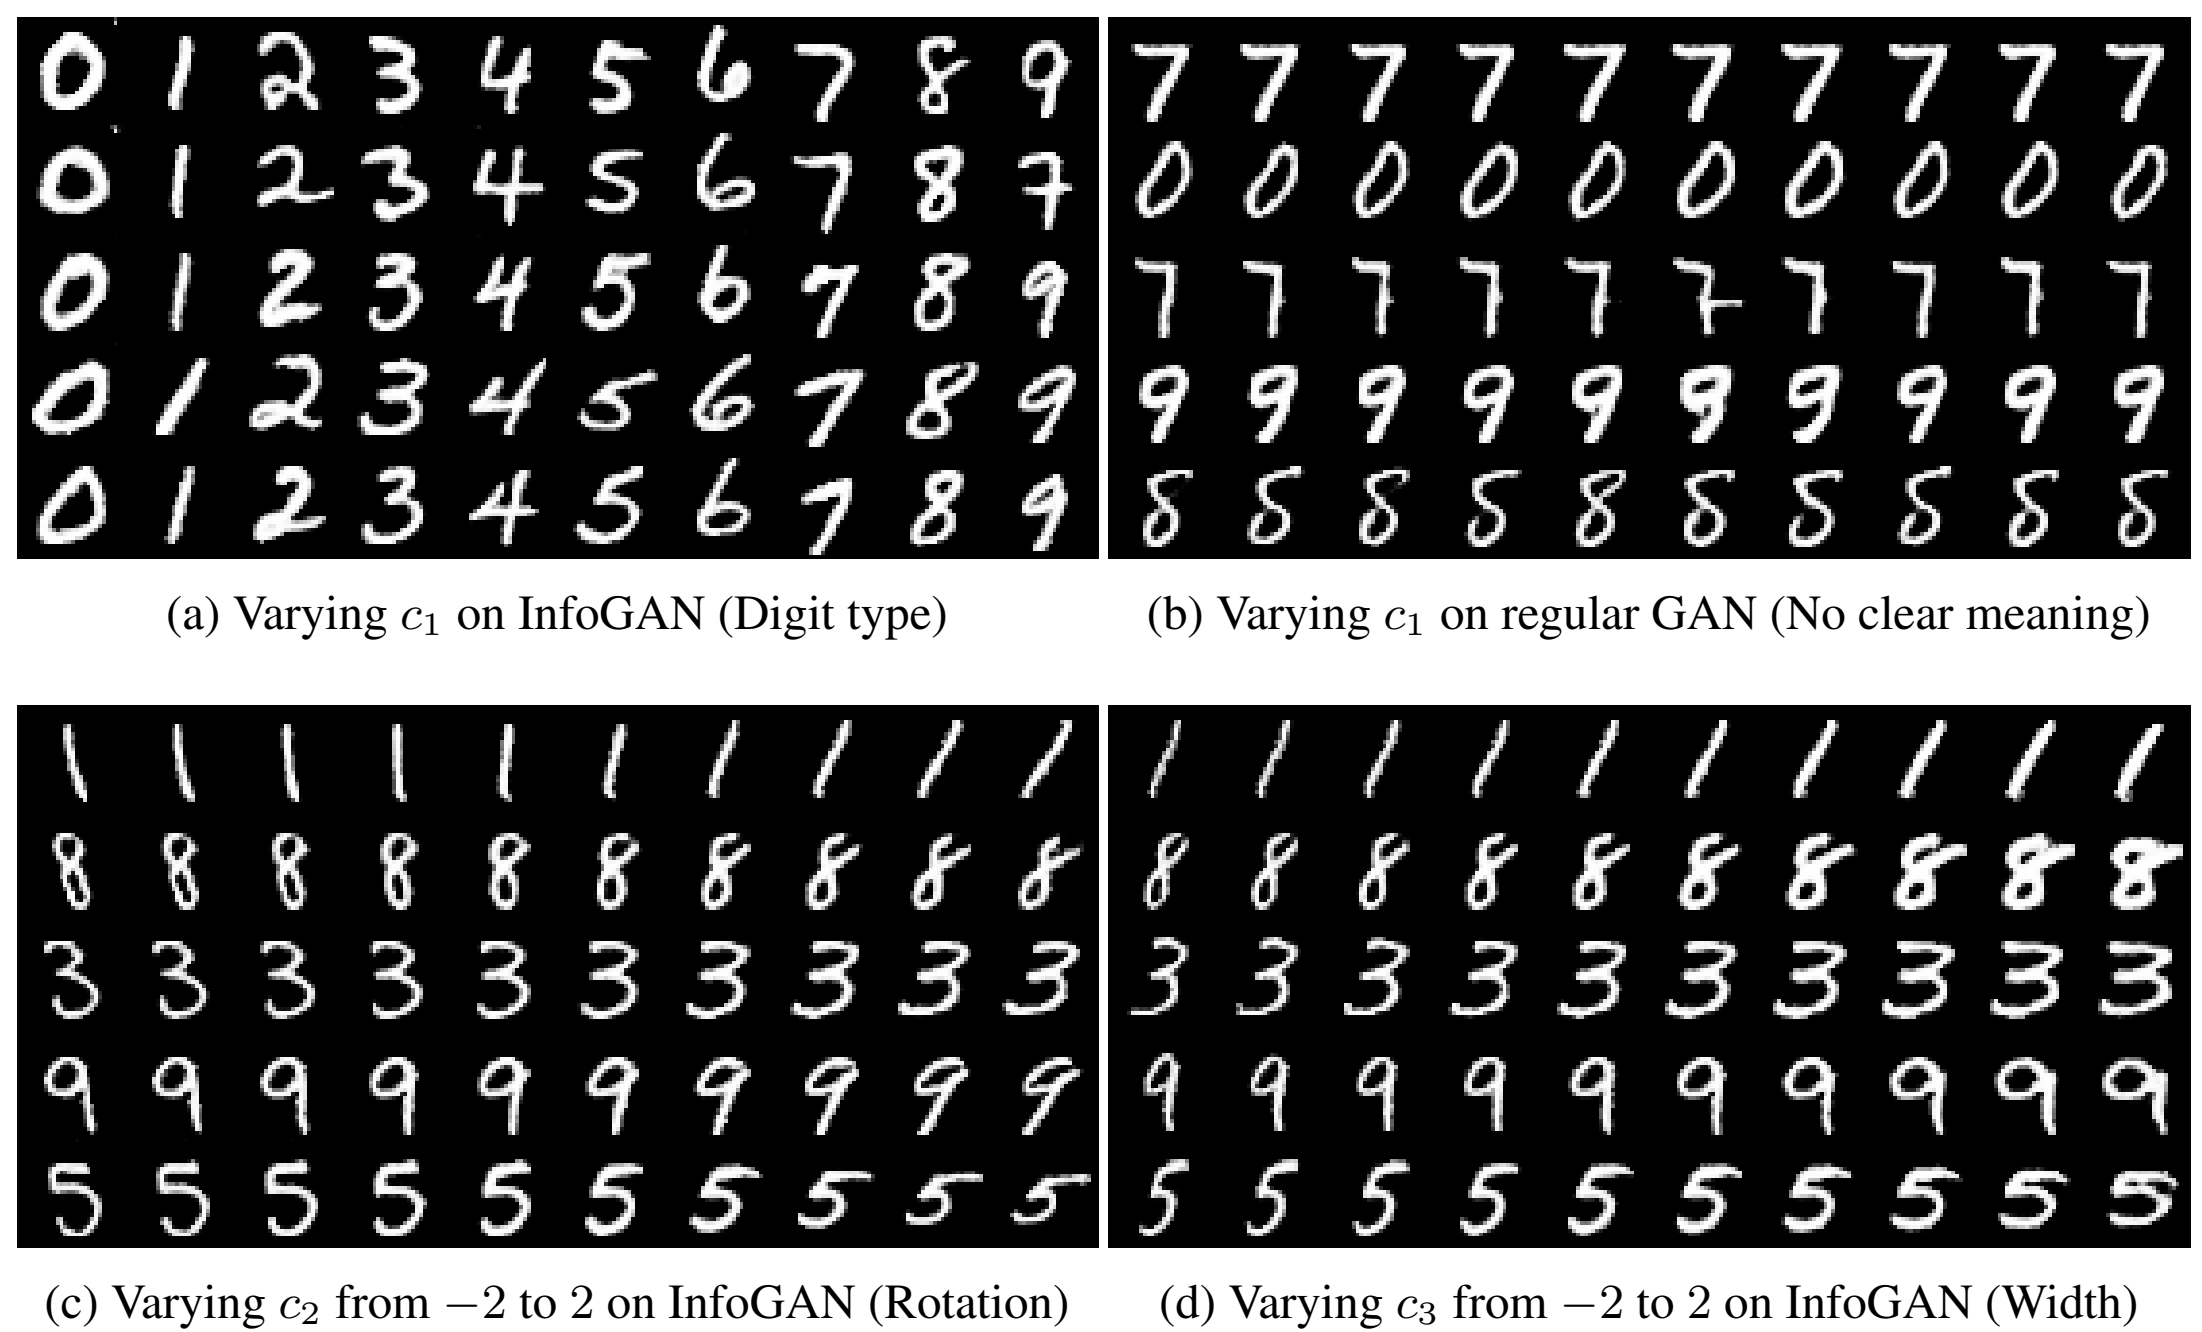
\includegraphics[width=\linewidth]{figs/infogan_mnist.png}
		\end{figure}
	\end{block}
	
	\myfootnotewithlink{https://arxiv.org/abs/1606.03657}{Chen X. et al. InfoGAN: Interpretable Representation Learning by Information Maximizing Generative Adversarial Nets, 2016}
\end{frame}
%=======
\begin{frame}{InfoGAN}
	\begin{block}{Latent codes on 3D Faces}
		\begin{figure}
			\centering
			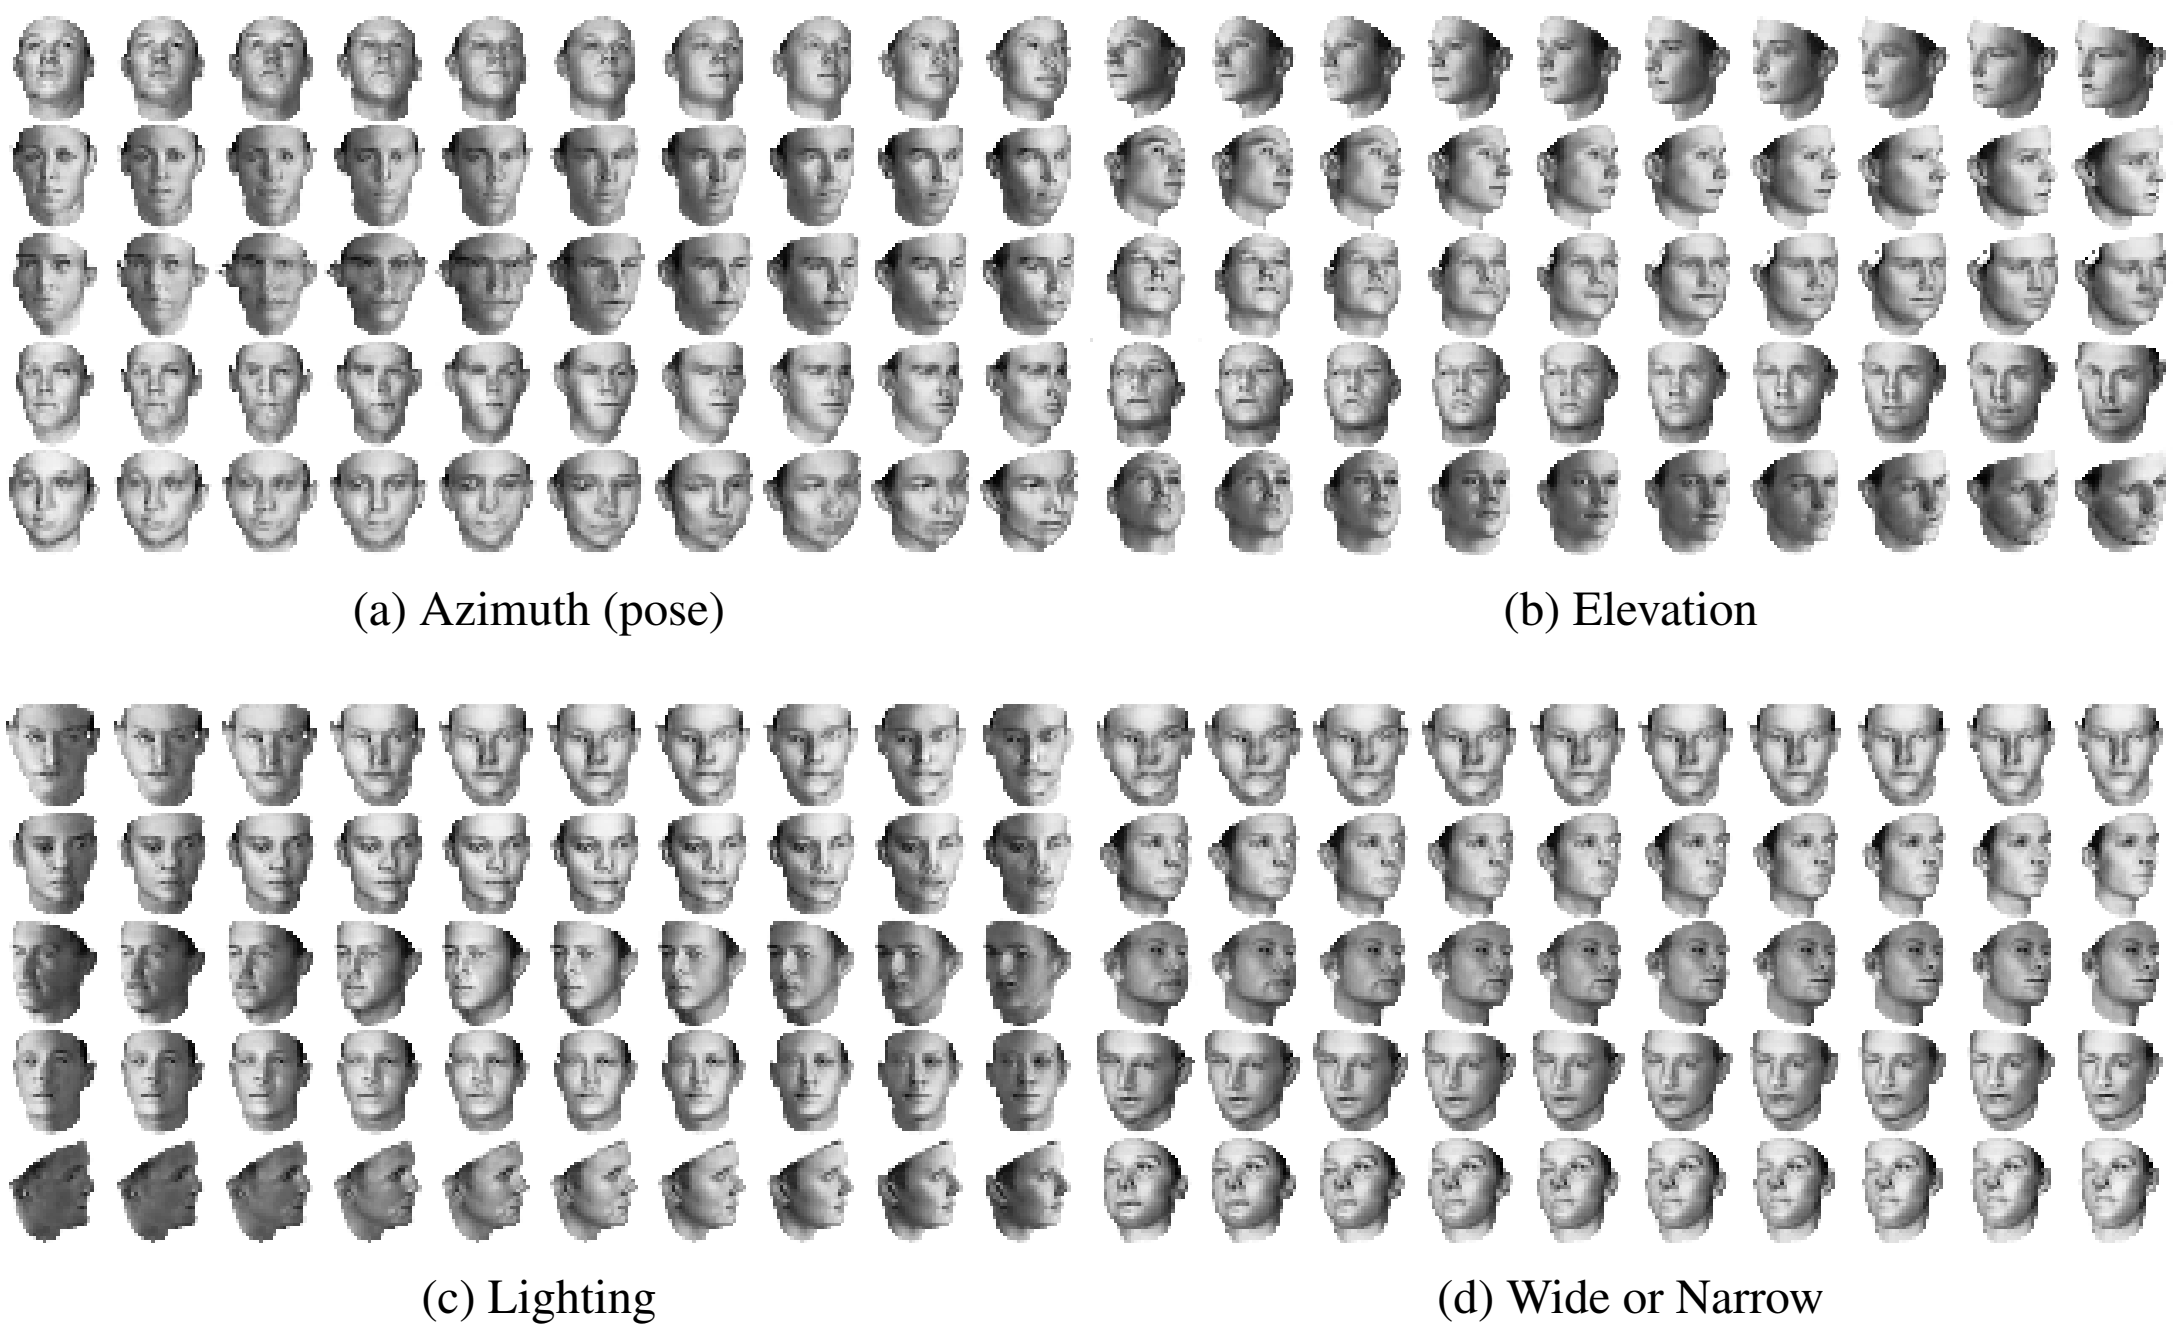
\includegraphics[width=\linewidth]{figs/infogan_faces.png}
		\end{figure}
	\end{block}
	
	\myfootnotewithlink{https://arxiv.org/abs/1606.03657}{Chen X. et al. InfoGAN: Interpretable Representation Learning by Information Maximizing Generative Adversarial Nets, 2016}
\end{frame}
%=======
\begin{frame}{$\beta$-VAE, Disentanglement metric}
\end{frame}
%=======
\begin{frame}{$\beta$-VAE}
	\begin{block}{Disentangling metric}
		\begin{enumerate}
			\item Generate two sets of objects
			\[
			\bx_{li} \sim \text{Sim}(\bv_{li}, \bw_{li}); \quad \bx_{lj} \sim \text{Sim}(\bv_{lj}, \bw_{lj}); \quad y_{ij} \sim U[1, d].
			\]
			\[
			\bv_{li} \sim p(\bv); \quad \bv_{lj} \sim p(\bv) \, ([v_{li}]_y = [v_{lj}]_y); \quad \bw_{li}, \bw_{lj} \sim p(\bw).
			\]
			\item Find representations
			\[
			q(\bz | \bx) = \mathcal{N}\left(\mu(\bx) | \sigma^2(\bx)\right); \quad \bz_{li} = \mu(\bx_{li}); \quad \bz_{lj} = \mu(\bx_{lj}).
			\]
			\item Use accuracy of classifier $p(y | \bz_{\text{diff}})$ with a low VC-dimension as metric of disentanglement
			\[
			\bz_{\text{diff}} = \frac{1}{L} \sum_{l=1}^L | \bz_{li} - \bz_{lj} |.
			\]
		\end{enumerate}
	\end{block}

	\myfootnotewithlink{https://openreview.net/references/pdf?id=Sy2fzU9gl}{Higgins I. et al. beta-VAE: Learning Basic Visual Concepts with a Constrained Variational Framework, 2017}
\end{frame}
%=======
\begin{frame}{$\beta$-VAE}
	\begin{itemize}
		\item \textbf{Top row:} original images.
		\item \textbf{Second row:} the corresponding reconstructions. 
		\item \textbf{Remaining rows:} latent traversals ordered by KL divergence with the prior. 
		\item \textbf{Heatmaps:} latent activations for each 2D position.
	\end{itemize}
	\begin{figure}
		\centering
		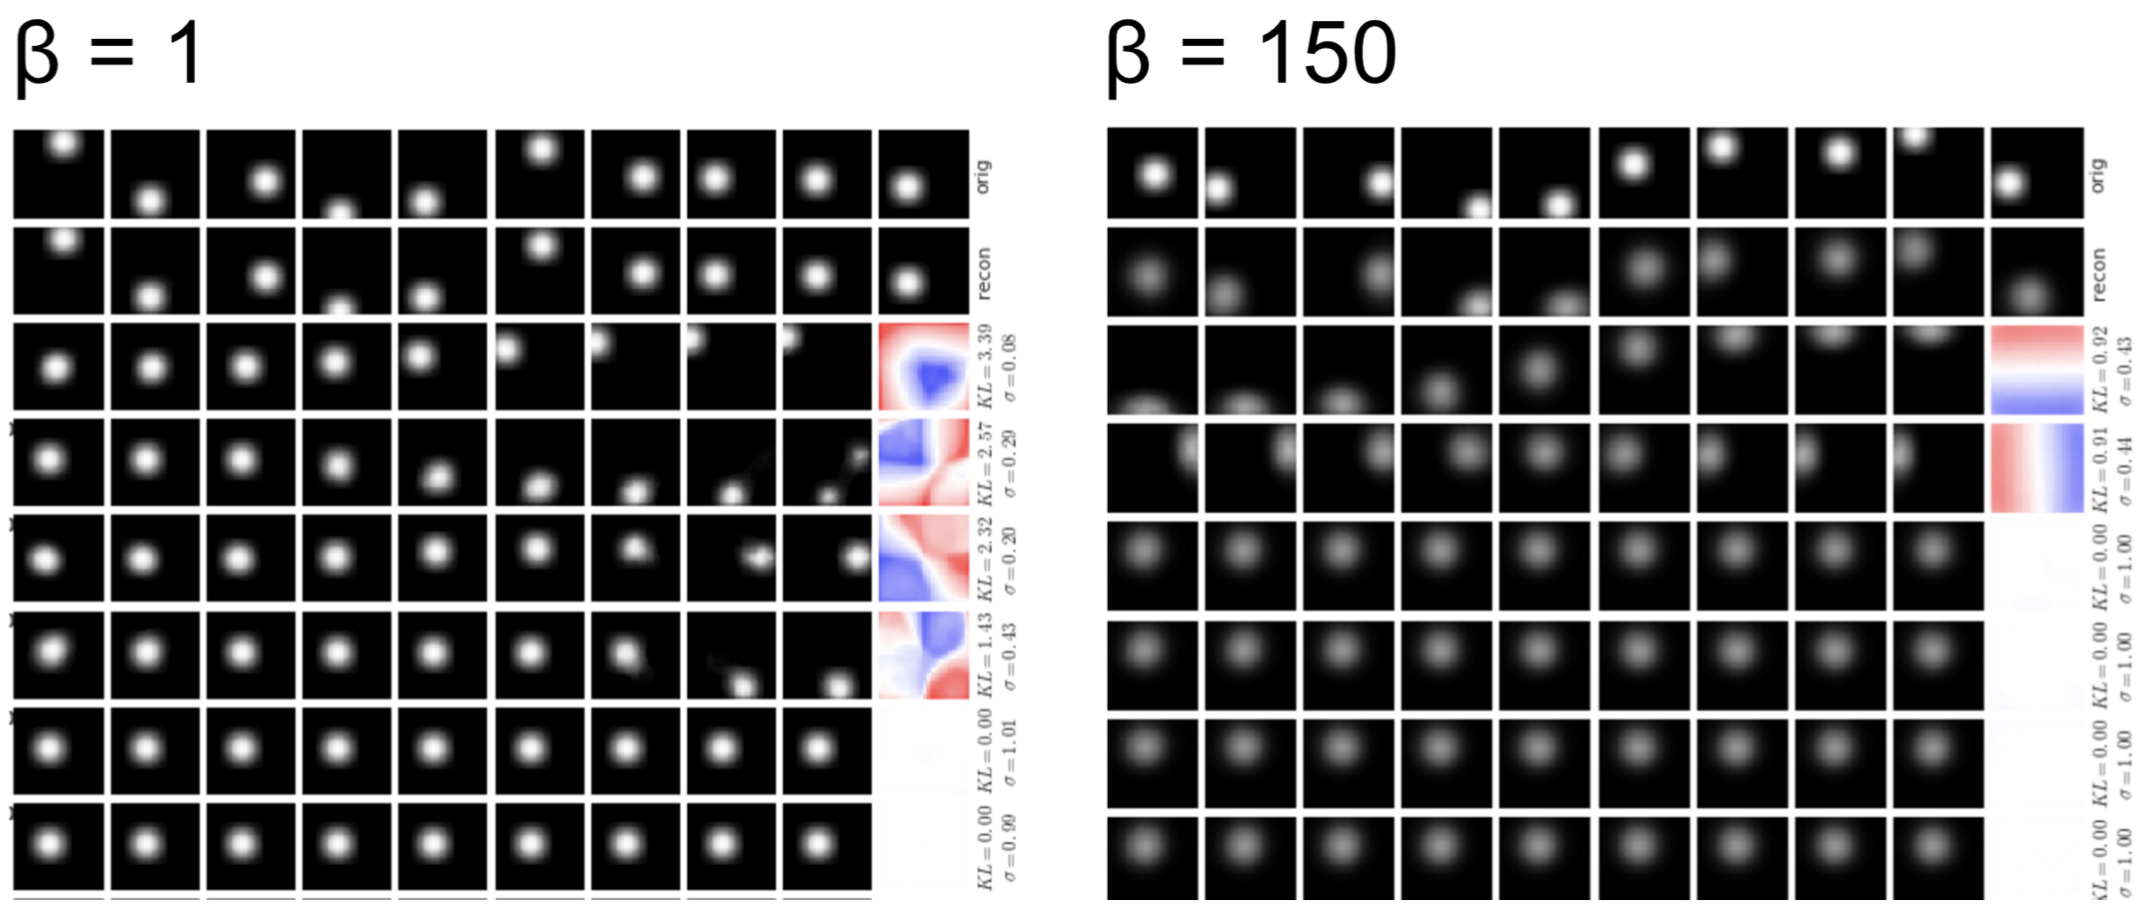
\includegraphics[width=\linewidth]{figs/betaVAE_6.png}
	\end{figure}

	\myfootnotewithlink{https://arxiv.org/abs/1804.03599}{Burgess C. P. et al. Understanding disentangling in $\beta$-VAE, 2018}
\end{frame}
%=======
\begin{frame}{$\beta$-VAE}
	\begin{block}{Controlled encoding capacity}
		\vspace{-0.5cm}
		\[
		\mathcal{L}(q, \btheta, \beta) = \mathbb{E}_{q(\bz | \bx)} \log p(\bx | \bz, \btheta) - | KL (q(\bz | \bx) || p(\bz)) - C|.
		\]
	\end{block}
	\begin{figure}
		\centering
		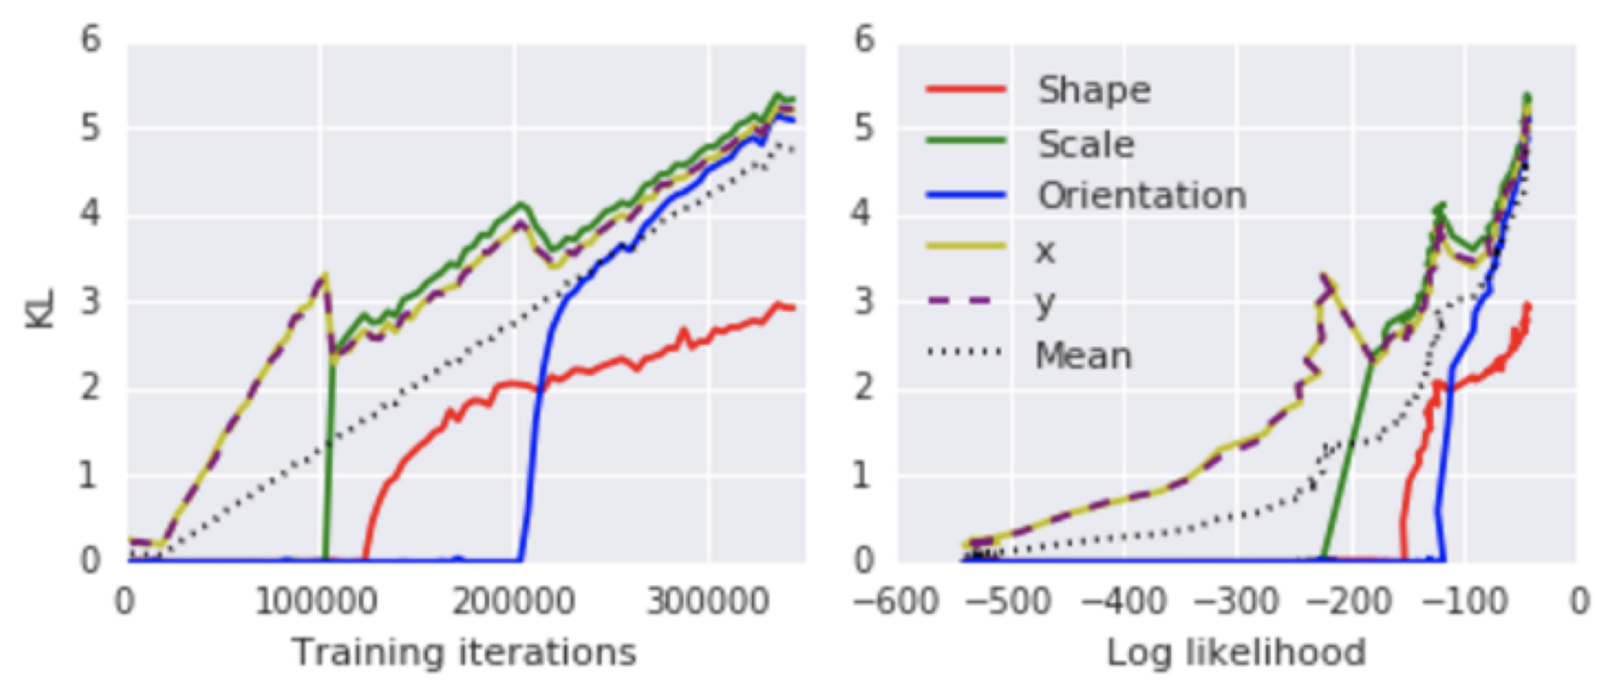
\includegraphics[width=0.9\linewidth]{figs/betaVAE_7.png}
	\end{figure}
	The early capacity is allocated to positional latents only, followed by a scale latent, then shape and orientation latents.
	
	\myfootnotewithlink{https://arxiv.org/abs/1804.03599}{Burgess C. P. et al. Understanding disentangling in $\beta$-VAE, 2018}
\end{frame}
%=======
\begin{frame}{$\beta$-VAE}
	\begin{block}{Controlled encoding capacity}
		\vspace{-0.5cm}
		\[
		\mathcal{L}(q, \btheta, \beta) = \mathbb{E}_{q(\bz | \bx)} \log p(\bx | \bz, \btheta) - | KL (q(\bz | \bx) || p(\bz)) - C|.
		\]
		\vspace{-0.5cm}
	\end{block}
	\begin{figure}
		\centering
		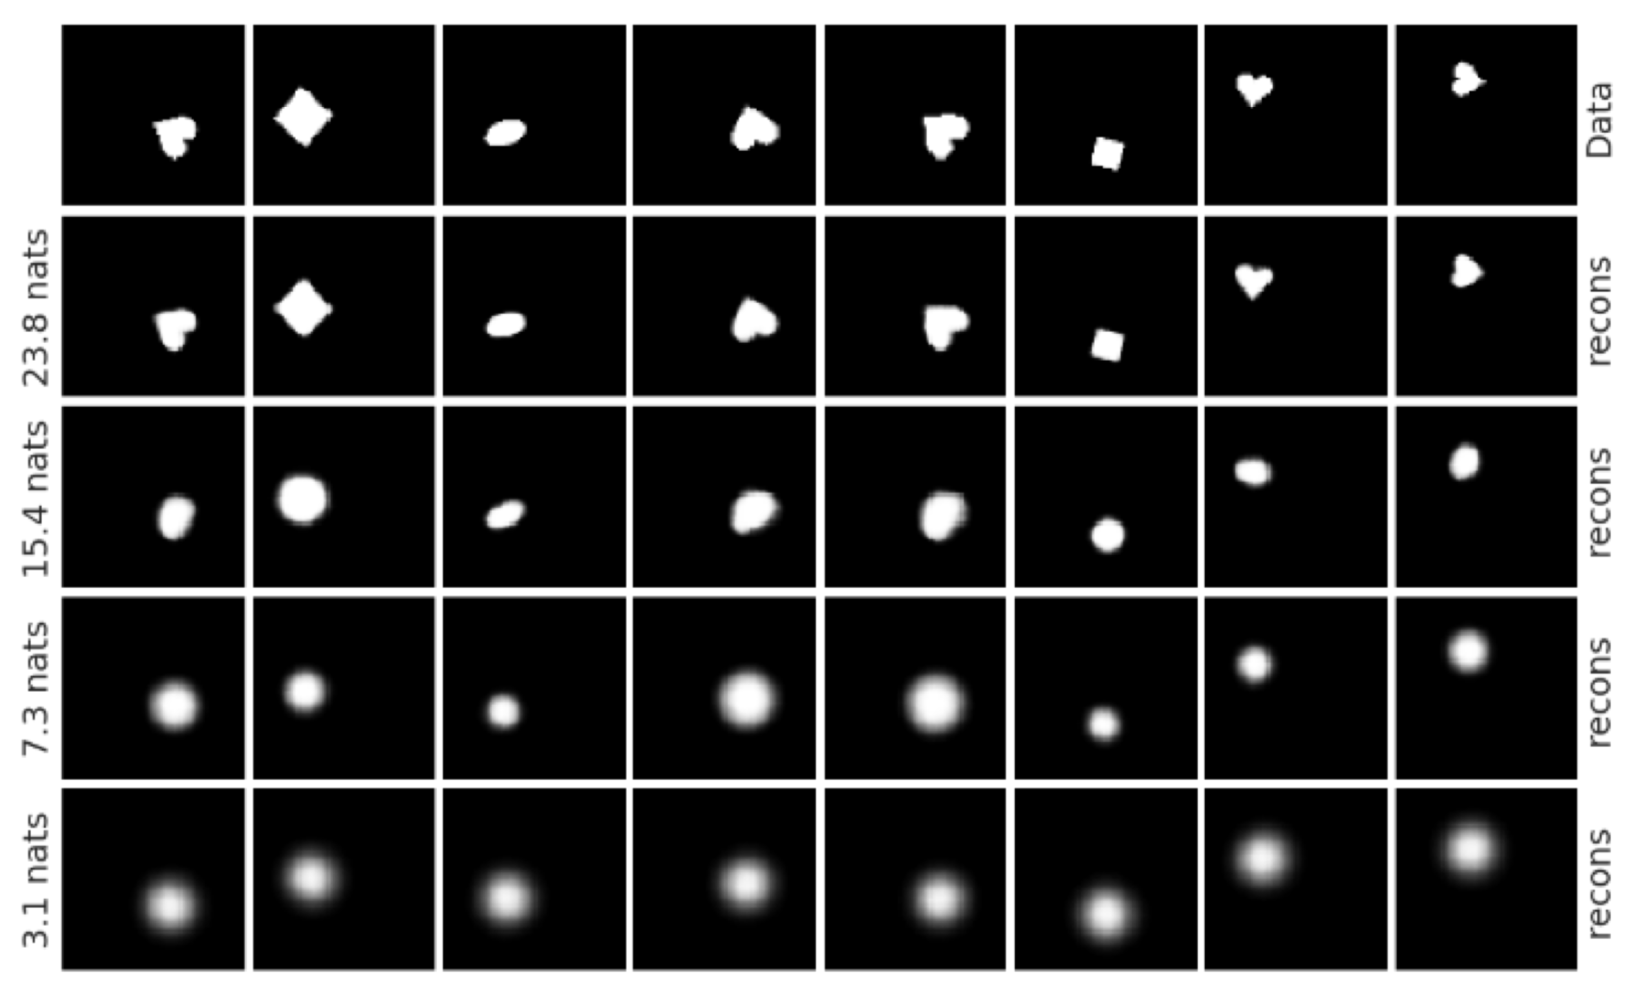
\includegraphics[width=0.7\linewidth]{figs/betaVAE_8.png}
	\end{figure}
	
	\myfootnotewithlink{https://arxiv.org/abs/1804.03599}{Burgess C. P. et al. Understanding disentangling in $\beta$-VAE, 2018}
\end{frame}
%=======
\begin{frame}{$\beta$-VAE}
	\begin{figure}
		\centering
		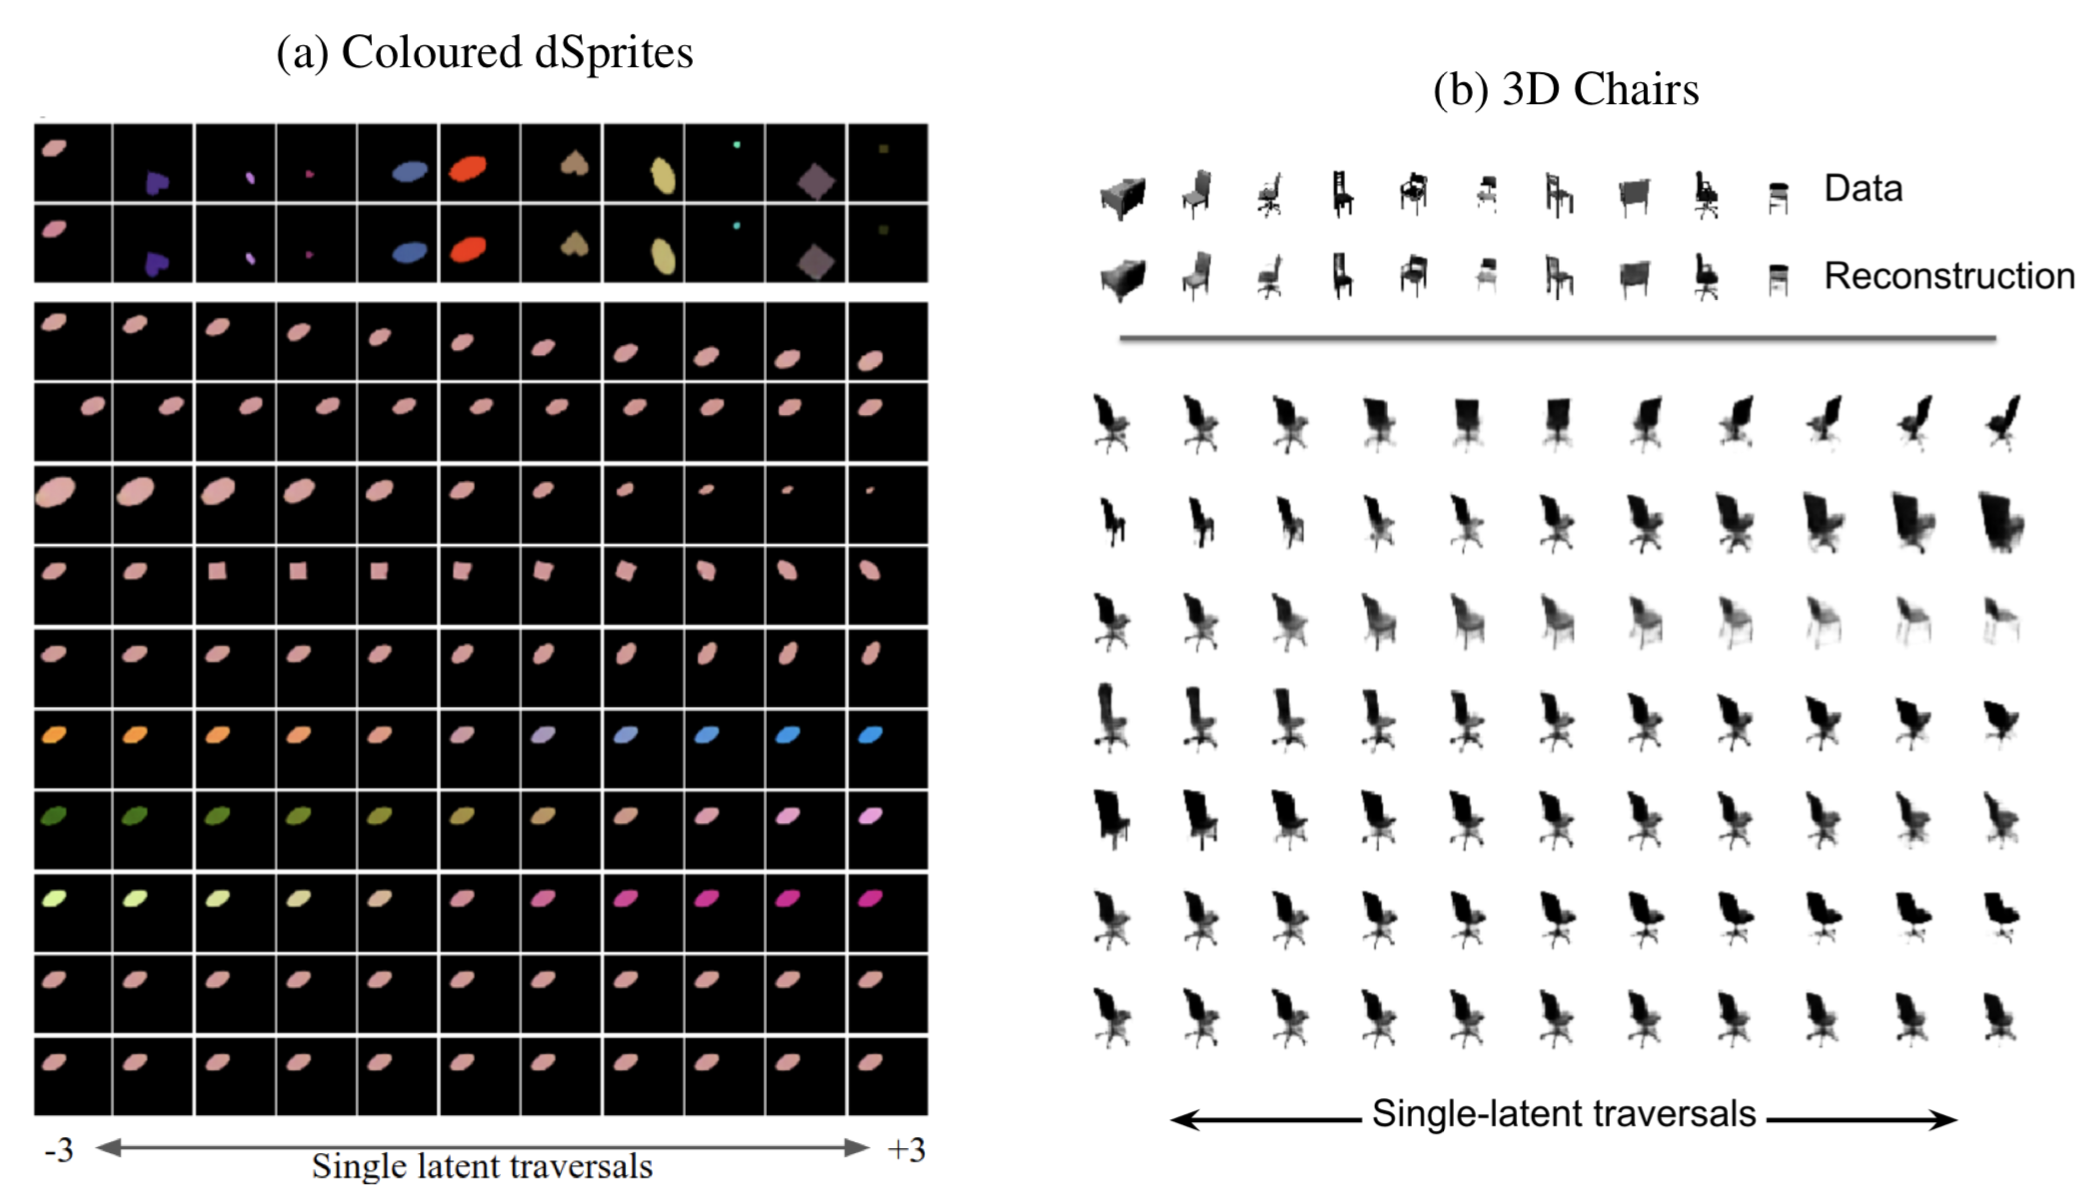
\includegraphics[width=1.0\linewidth]{figs/betaVAE_9.png}
	\end{figure}
	
	\myfootnotewithlink{https://arxiv.org/abs/1804.03599}{Burgess C. P. et al. Understanding disentangling in $\beta$-VAE, 2018}
\end{frame}
%=======
\begin{frame}{FactorVAE}
\end{frame}
%=======
\begin{frame}{FactorVAE}
	\begin{block}{Disentangled aggregated variational posterior}
		\vspace{-0.3cm}
		\[
			q(\bz) = \frac{1}{n} \sum_{i=1}^n q(\bz | \bx) = \prod_{j=1}^d q(z_j)
		\]
		\vspace{-0.3cm}
	\end{block}
	\begin{block}{Total correlation regularizer}
		\vspace{-0.3cm}
		\[
		\min KL(q(\bz) || \prod_{j=1}^d q(z_j))
		\]
		\vspace{-0.3cm}
	\end{block}
	\begin{block}{FactorVAE objective}
		\vspace{-0.3cm}
		\[
		\min_{\bphi, \btheta} \cL(\bphi, \btheta) - \gamma \cdot KL(q(\bz) || \prod_{j=1}^d q(z_j))
		\]
		\vspace{-0.3cm}
	\end{block}
	\begin{itemize}
		\item The last term is intractable.
		\item FactorVAE uses density ratio trick for estimation. 
	\end{itemize}

	\myfootnotewithlink{https://arxiv.org/abs/1802.05983}{Kim H., Mnih A. Disentangling by Factorising, 2018}
\end{frame}
%=======
\begin{frame}{FactorVAE}
	Consider two distributions $q_1(\bx)$, $q_2(\bx)$ and probilistic model
	\[
		p(\bx | y) = \begin{cases}
			q_1(\bx), \text{ if } y = 1, \\
			q_2(\bx), \text{ if } y = 0,
		\end{cases}
		\quad 
		y \sim \text{Bern}(0.5).
	\]
	\begin{block}{Density ratio trick}
		\vspace{-0.5cm}
		\begin{multline*}
			\frac{q_1(\bx)}{q_2(\bx)} = \frac{p(\bx | y = 1)}{p(\bx | y = 0)} = \frac{p(y = 1 | \bx) p(\bx)}{p(y=1)} \bigg/ \frac{p(y = 0 | \bx) p(\bx)}{p(y=0)} = \\
			= \frac{p(y = 1 | \bx)}{p(y = 0 | \bx)} = \frac{p(y = 1 | \bx)}{1 - p(y = 1 | \bx)} = \frac{D(\bx)}{1 - D(\bx)}
		\end{multline*}
	Here $D(\bx)$ could be treated as a discriminator a model the output of which is a probability that $\bx$ is a sample
	from $q_1(\bx)$ rather than from $q_2(\bx)$.
	\end{block}

	\myfootnotewithlink{https://arxiv.org/abs/1802.05983}{Kim H., Mnih A. Disentangling by Factorising, 2018}
\end{frame}
%=======
\begin{frame}{FactorVAE}
	
	\begin{block}{FactorVAE objective}
		\vspace{-0.3cm}
		\[
		\min_{\btheta, \bphi} \text{ELBO}(\btheta, \bphi) - \gamma \cdot KL(q(\bz) || \prod_{j=1}^d q(z_j))
		\]
		\vspace{-0.3cm}
	\end{block}
	
	\begin{block}{Total correlation regularizer}
		\vspace{-0.7cm}
		\begin{multline*}
		KL(q(\bz) || \prod_{j=1}^d q(z_j)) = KL(q(\bz) || \bar{q}(\bz)) = \\ =\bbE_{q(\bz)} \log \frac{q(\bz)}{\bar{q}(\bz)} \approx \bbE_{q(\bz)} \log \frac{D(\bz)}{1 - D(\bz)}
		\end{multline*}
		\vspace{-0.3cm}
	\end{block}
	VAE and GAN are trained simultaneously.

	\myfootnotewithlink{https://arxiv.org/abs/1802.05983}{Kim H., Mnih A. Disentangling by Factorising, 2018}
\end{frame}
%=======
\begin{frame}{FactorVAE}
	
	\begin{minipage}[t]{0.5\columnwidth}
		\begin{figure}
			\centering
			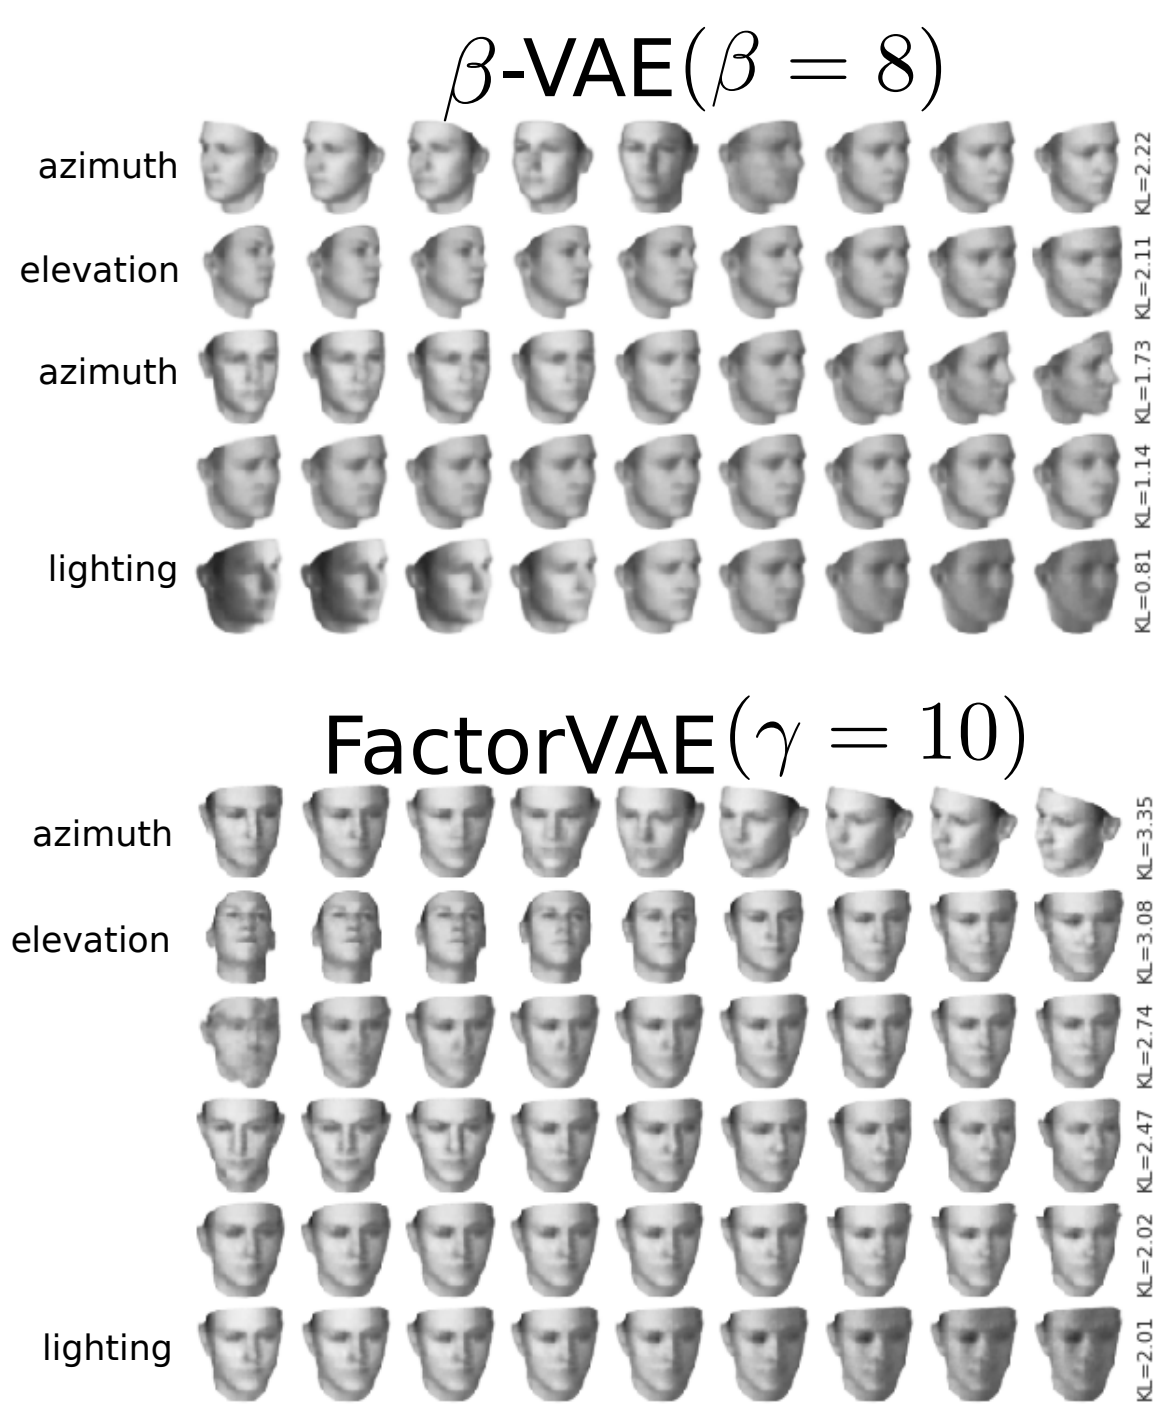
\includegraphics[width=\linewidth]{figs/factorvae_1}
		\end{figure}
	\end{minipage}%
	\begin{minipage}[t]{0.5\columnwidth}
		\vspace{1.7cm}
		\begin{figure}[h]
			\centering
			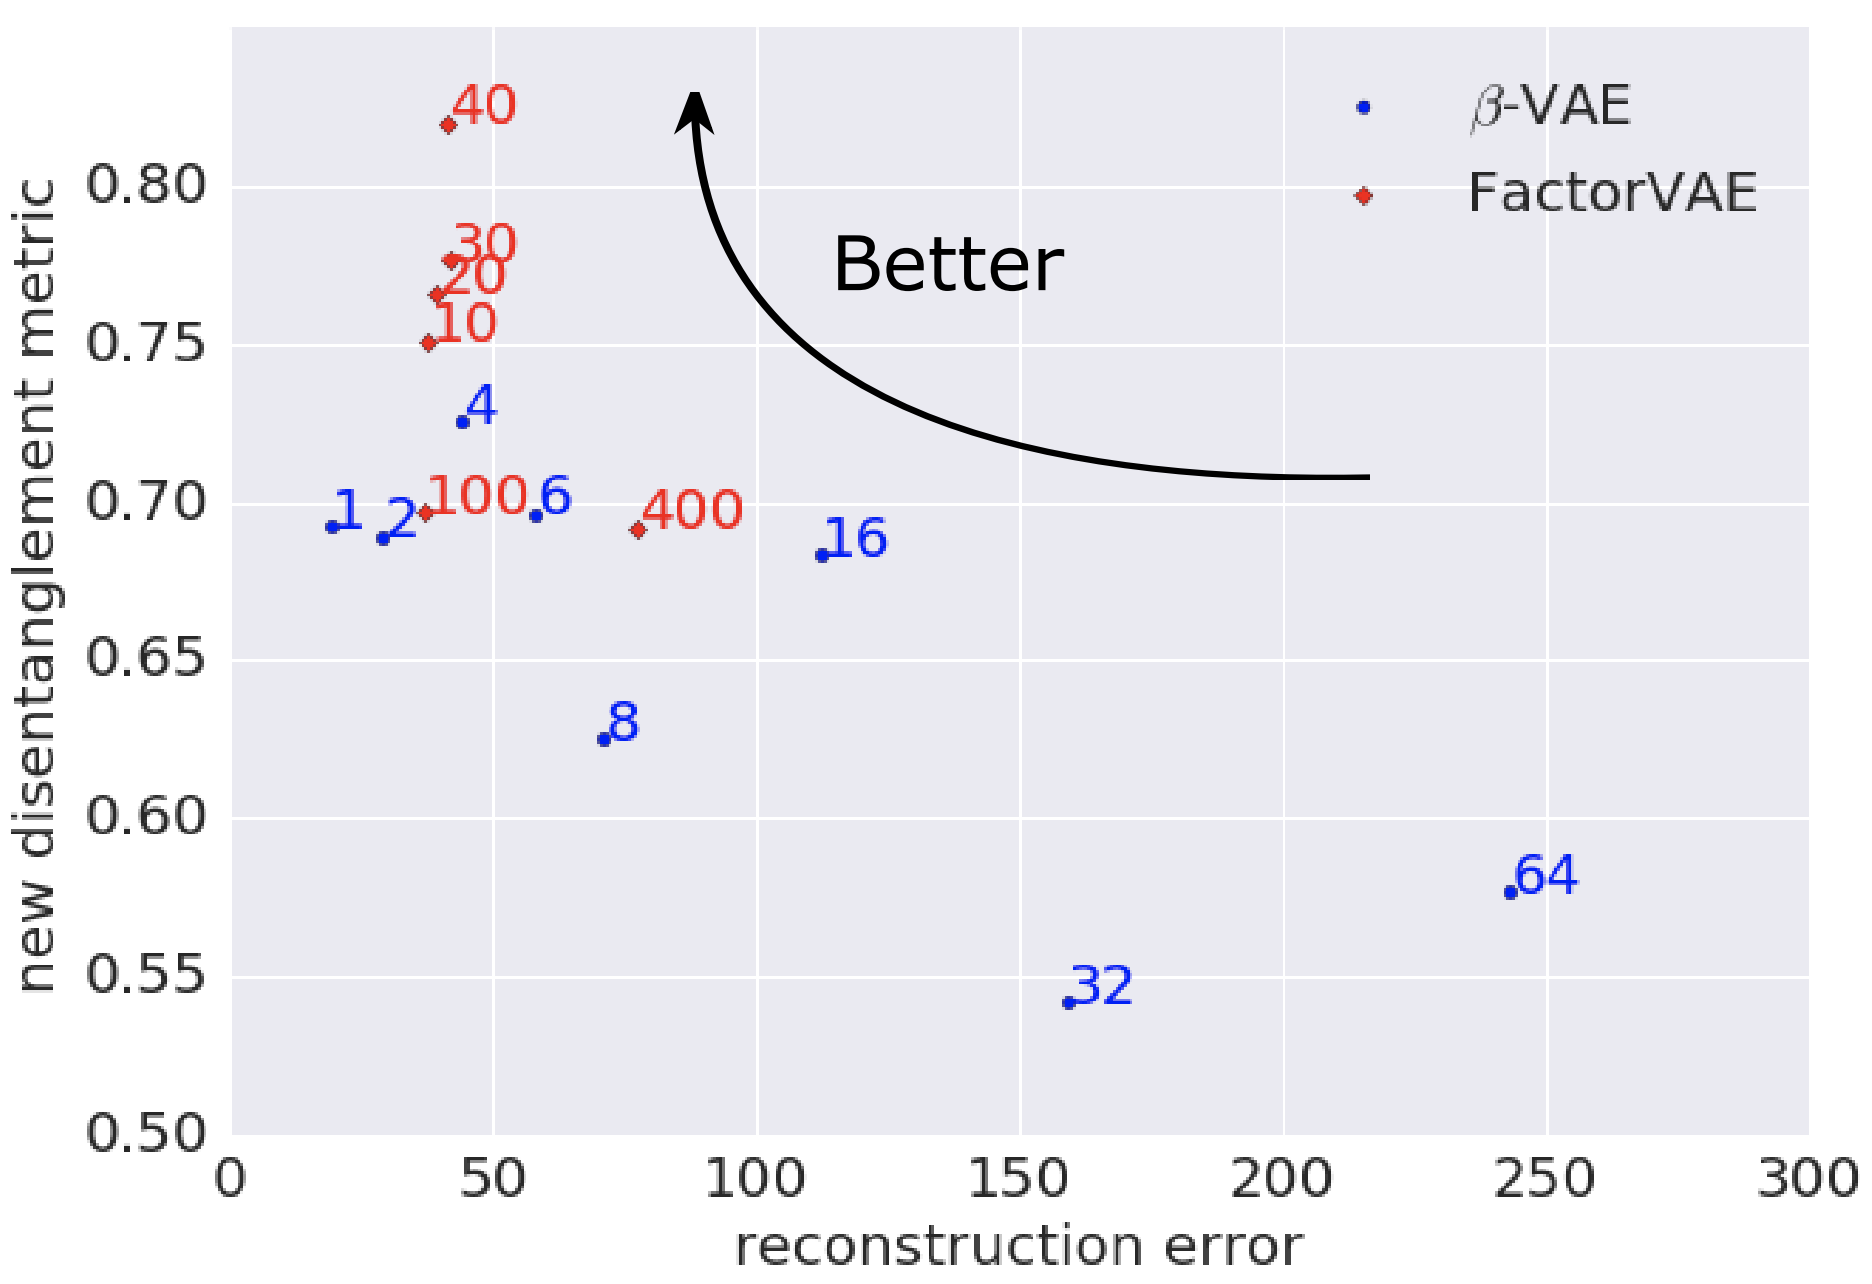
\includegraphics[width=\linewidth]{figs/factorvae_2}
		\end{figure}
	\end{minipage}

	\myfootnotewithlink{https://arxiv.org/abs/1802.05983}{Kim H., Mnih A. Disentangling by Factorising, 2018}
\end{frame}
%=======
\begin{frame}{Improved techniques for training GANs}
\end{frame}
%=======
\begin{frame}{Improved techniques for training GANs}
	\begin{itemize}
		\item Feature matching
		\[
			\cL_G = \| \bbE_{\pi(\bx)} \mathbf{d}(\bx) - \bbE_{p(\bz)} \mathbf{d}(G(\bz)) \|_2^2
		\]
		Here $\mathbf{d}(\bx)$ -- intermediate layer of discriminator. Matching the learned discriminator statistics instead of the output of the discriminator. Helps to avoid the vanishing gradients for sufficiently good discriminator.
		\item Historical averaging adds extra loss term for generator and discriminator losses
		\vspace{-0.2cm}
		\[
		 \| \btheta - \frac{1}{T}\sum_{t=1}^T \btheta_t\|^2_2.
		\]
		Here $\btheta_t$ -- value of parameters at the previous step $t$. It allows to stabilize training procedure.
	\end{itemize}
	\myfootnotewithlink{https://arxiv.org/abs/1606.03498}{Salimans T. et al. Improved Techniques for Training GANs, 2016}
\end{frame}
%=======
\begin{frame}{Improved techniques for training GANs}
	\begin{itemize}
		\item One-sided label smoothing. Instead of using one-hot labels in classification, use $(1 - \alpha)$ for real data (the generated samples are not smoothed).
		\[
			D^*(\bx) = \frac{(1 - \alpha )\pi(\bx)}{\pi(\bx) + p(\bx | \btheta)}
		\]
		\item Virtual batch normalization. BatchNorm makes samples within minibatch are highly correlated.
		\begin{figure}
			\centering
			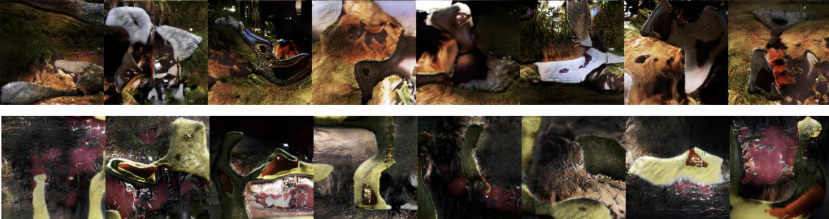
\includegraphics[width=0.6\linewidth]{figs/virtual_batch_norm}
		\end{figure}
	Use reference fixed batch to compute the normalization statistics. To avoid overfitting construct batch with the reference batch and the current sample. 
	\end{itemize}
	\myfootnotewithlink{https://arxiv.org/abs/1606.03498}{Salimans T. et al. Improved Techniques for Training GANs, 2016}
\end{frame}
%=======
\end{document} 